\chapter{Two-fluid physical modeling\label{sec:phyical_modeling}}

This chapter details the physical models for the Two-fluid approach. First, the definition of fluid properties is defined using two methods, through the dataset (section~\ref{sec:fluid_properties} and through an external software (section~\ref{sec:fluid-prop-ext}). Then the interfacial forces are described in section~\ref{sec:interfa-forces}. Some particular source terms for the momentum (section~\ref{sec:analytical}) and the mass equations (section~\ref{sec:injection}). The management of the dispersed phase diameter is described in section~\ref{sec:diam-mgmt}.

%%%
\section{Fluid proprieties\label{sec:fluid_properties}}
\subsection{Basic proprieties of fluid}
The domain used for the different phases must be defined by a medium characterized by one or more fluid subdomains of different properties. This composite environment is defined by \texttt{Milieu\_composite}.\\
The models aims to give the basic proprieties of fluids such as :
\begin{itemize}
    \item[\small \textcolor{blue}{\ding{109}}] Kinematic viscosity $\mu$
    \item[\small \textcolor{blue}{\ding{109}}] Density $\rho$
    \item[\small \textcolor{blue}{\ding{109}}] Thermal diffusivity $\alpha$
    \item[\small \textcolor{blue}{\ding{109}}] Conductivity $\lambda$
    \item[\small \textcolor{blue}{\ding{109}}] Calorific capacity $Cp$
    \item[\small \textcolor{blue}{\ding{109}}] Thermal dilatation coefficient $\beta_{co}$
\end{itemize}
The model is implemented in \texttt{Fluide_reel_base} as 
\begin{lstlisting}[language=c++]
void Fluide_reel_base::set_param(Param& param)
{
  param.ajouter("T_ref", &T_ref_);
  param.ajouter("P_ref", &P_ref_);
  set_additional_params(param);
}
\end{lstlisting}
The fluid proprieties operator must fill following tabs :
\begin{itemize}
   \item[\small \textcolor{blue}{\ding{109}}] \texttt{rho\textunderscore} density
   \item[\small \textcolor{blue}{\ding{109}}] \texttt{dP\textunderscore rho\textunderscore} density derivative regarding pressure
   \item[\small \textcolor{blue}{\ding{109}}] \texttt{dT\textunderscore rho\textunderscore} density derivative regarding temperature
   \item[\small \textcolor{blue}{\ding{109}}] \texttt{h\textunderscore} enthalpy
   \item[\small \textcolor{blue}{\ding{109}}] \texttt{dP\textunderscore h\textunderscore} enthalpy derivative regarding pressure
   \item[\small \textcolor{blue}{\ding{109}}] \texttt{dT\textunderscore h\textunderscore} enthalpy derivative regarding temperature
   \item[\small \textcolor{blue}{\ding{109}}] \texttt{cp\textunderscore} heat capacity
   \item[\small \textcolor{blue}{\ding{109}}] \texttt{beta\textunderscore} thermal dilatation coefficient
   \item[\small \textcolor{blue}{\ding{109}}] \texttt{mu\textunderscore} kinematic viscosity
   \item[\small \textcolor{blue}{\ding{109}}] \texttt{lambda\textunderscore} conductivity
\end{itemize}

%%%
\subsubsection{Non-compressible fluid}
The model is implemented in \texttt{Fluide\_Incompressible} (from TRUST incompressible) :
\begin{lstlisting}[language=c++]
void Fluide_Incompressible::set_param(Param& param)
{
  Fluide_base::set_param(param);
  //La lecture de rho est rendue obligatoire ici
  param.supprimer("rho");
  param.ajouter("rho",&rho,Param::REQUIRED);
}
\end{lstlisting}
This class allows to give the proprieties previously introduced (or are set to $0$) but with a density that is mandatory. Let's notice that here neither the density nor the specific heat can be a \texttt{Champ_Uniforme}.

%%%
\subsubsection{Sodium gas}
The model is implemented in \texttt{Fluide\_sodium\_gaz} :
\begin{lstlisting}[language=c++]
void Fluide_sodium_gaz::set_param(Param& param)
\end{lstlisting}
The model implemented reads \texttt{Lois\_sodium.h} and writes:
\begin{itemize}
   \item[\small \textcolor{blue}{\ding{109}}] { "temperature", { 371 - 273.15, 2503.7 - 273.15 } }, //Tri-critical point temperature { "pression", { 4.127e-6, 260e5 } };                // Associated pressure
\end{itemize}

%%%
\subsubsection{Sodium liquid}
The model is implemented in \texttt{Fluide\_sodium\_liquide}:
\begin{lstlisting}[language=c++]
void Fluide_sodium_liquide::set_param(Param& param)
\end{lstlisting}
The model implemented reads \texttt{Lois\_sodium.h} and writes:
\begin{itemize}
  \item[\small \textcolor{blue}{\ding{109}}] { "temperature", { 371 - 273.15, 2503.7 - 273.15 } }; //de la temperature de solidification au pt tricritique
\end{itemize}

%%%
\subsubsection{Stiffened gas}
The model is implemented in \texttt{Fluide\_stiffened\_gas}:
\begin{lstlisting}[language=c++]
void Fluide_stiffened_gas::set_param(Param& param)
{
  Fluide_reel_base::readOn(is);
  if (Cv_ == -1.) Cv_ = R_ / (gamma_ - 1.0);
  return is;
}
void Fluide_stiffened_gas::set_param(Param& param)
{
  Fluide_reel_base::set_param(param);
  param.ajouter("gamma",&gamma_); // Heat ratio
  param.ajouter("pinf",&pinf_); // Reference pressure in law
  param.ajouter("mu",&mu__); // viscosity
  param.ajouter("lambda",&lambda__); // conductivity
  param.ajouter("Cv",&Cv_); // heat capacity
  param.ajouter("q",&q_); 
  param.ajouter("q_prim",&q_prim_);
}
\end{lstlisting}
The model implemented is:
\begin{itemize}
  \item[\small \textcolor{blue}{\ding{109}}] \texttt{rho\textunderscore} $=\frac{p+\texttt{pinf\textunderscore}}{\left(\texttt{gamma\textunderscore} -1.0\right)\left(T+\num{273.15}\right)\texttt{Cv\textunderscore}}$, the density
  \item[\small \textcolor{blue}{\ding{109}}] \texttt{dP\textunderscore rho\textunderscore} $=\frac{1.0}{\left(\texttt{gamma\textunderscore} -1.0\right)\left(T+\num{273.15}\right)\left(\texttt{Cv\textunderscore} \right)}$, the density derivative regarding pressure
  \item[\small \textcolor{blue}{\ding{109}}] \texttt{dT\textunderscore rho\textunderscore}$ =-\frac{p+\texttt{pinf\textunderscore}}{\left(\texttt{gamma\textunderscore} - 1.0\right)\left(T+\num{273.15}\right)^2\texttt{Cv\textunderscore}}$, the density derivative regarding temperature
  \item[\small \textcolor{blue}{\ding{109}}] \texttt{h\textunderscore } $=\texttt{ gamma\textunderscore Cv\textunderscore}\left(T+\num{273.15}\right)+\texttt{q\textunderscore}$, the enthalpy
  \item[\small \textcolor{blue}{\ding{109}}] \texttt{dP\textunderscore h\textunderscore} $=0.$, the enthalpy derivative regarding pressure
  \item[\small \textcolor{blue}{\ding{109}}] \texttt{dT\textunderscore h\textunderscore}$ = \texttt{cp\textunderscore} \left(T,P\right)$, the enthalpy derivative regarding temperature
  \item[\small \textcolor{blue}{\ding{109}}] \texttt{cp\textunderscore} $ = \texttt{gamma\textunderscore Cv\textunderscore}$, the heat capacity
  \item[\small \textcolor{blue}{\ding{109}}] \texttt{beta\textunderscore}$ = \frac{1.0}{T+\num{273.15}}$
  \item[\small \textcolor{blue}{\ding{109}}] \texttt{mu\textunderscore}$ = \texttt{mu\textunderscore \textunderscore}$
  \item[\small \textcolor{blue}{\ding{109}}] \texttt{lambda\textunderscore}$ = \texttt{lambda\textunderscore \textunderscore}$
\end{itemize}

%%%
\subsubsection{R12_C1 and Eau_c3}
The models are implemented in \texttt{Fluide\_R12\_c1\_liquide}, \texttt{Fluide\_R12\_c1\_gaz}, \texttt{Fluide\_eau\_c3\_liquide} and \texttt{Fluide\_eau\_c3\_gaz}. The low boiling of refrigerant R12 (dichlorodifluoromethane) mimics Pressurized water reactor dimensionless numbers. Those values are available in Cathare code.
For example, in \textcite{KREPPER20113851}, one can find : \\
\begin{center}
\begin{tabular}{c c c } 
\toprule
Fluid & Water & R12 \\ \midrule
\rowcolor[gray]{0.9} Pressure [bar] & $155$ & $26$ \\  
$T_{sat}$ [\textdegree C] &  $344.9$ &  $86.5$ \\ 
\rowcolor[gray]{0.9} $\rho_{liquid}$ [kg/m3] &  $594.4$ & $1019.3$ \\ 
$Cp_{liquid}$ [kJ/kg] &  $8.950$ & $1.413$ \\ 
\rowcolor[gray]{0.9} $\lambda_{liquid}$ [W/m/K] & $0.472$ & $0.0458$ \\ 
$\mu_{liquid}$ [W/m/K] & $6.82 \times 10^{-5}$ & $9.23 \times 10^{-5}$ \\ 
\rowcolor[gray]{0.9} $\rho_{steam}$ [kg/m3] & $101.9$ & $170.7$ \\ 
$Cp_{steam}$ [kJ/kg] & $14.0$ & $1.281$\\ 
\rowcolor[gray]{0.9} $\lambda_{steam}$ [W/m/K] &  $0.126$ &  $0.0175$\\ 
$\mu_{steam}$ [W/m/K] & $2.30 \times 10^{-5}$ & $1.57 \times 10^{-5} $ \\ 
\rowcolor[gray]{0.9} $\sigma$ [J/m2] & $4.65 \times 10^{-3}$ & $1.80 \times 10^{-3}$ \\
$L_{vap}$ [kJ/kg] & $966.2$ & $86.48$ \\ \bottomrule 
\end{tabular}
\end{center}

%%%
\subsubsection{MUSIG fluid and medium}
In homogeneous MUlti-SIze Group (MUSIG), a distribution of bubbles or droplets between $r_{min}$ and $r_{max}$ is characterized by a statistical law (linear, exponential or log) and its discretization in $n$ sub groups with the same velocity, as depicted in Figures \ref{msgdis} from \textcite{cheung}.
\begin{figure}[!ht]
    \centering
    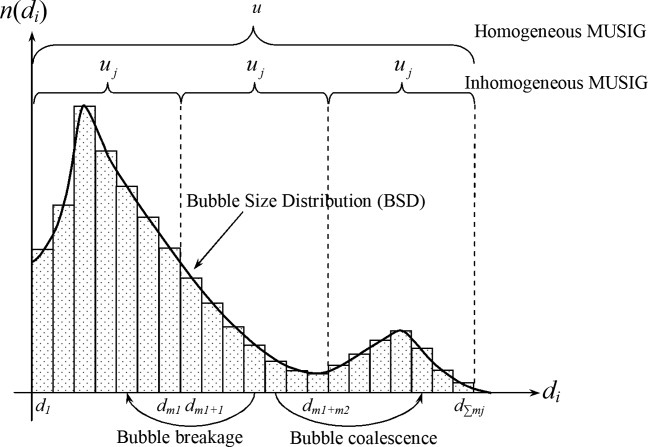
\includegraphics[scale =0.8]{Figure/musigdistri.jpg}
    \caption{Schema of the standard MUSIG and i-MUSIG models. In MUSIG, all size groups move with the same velocity field, whereas i-MUSIG displays an arbitrary number of velocity groups.}
    \label{msgdis}
\end{figure}
All bubbles from sub groups share the same velocity as the velocity of the mean Sauter diameter of the distribution $D_{sm}$. Thus, they share the same common total void fraction equation (mass), velocity (momentum equation) and temperature, allowing to compute only one common set of equations (mass, momentum and energy) with new source terms linked to the changes in the distribution (dilatability, coalescence, break-up).\\
The model is implemented in \texttt{Fluide\_MUSIG} and \texttt{Milieu\_MUSIG} :
\begin{lstlisting}[language=c++]
void Fluide_MUSIG::set_param(Param& param)
{
if(Motcle(mot) == "NBPHASES")
if (Motcle(mot) == "RMIN")
if (Motcle(mot) == "RMAX")
if(Motcle(mot) == "DIAMETRES" || Motcle(mot) == "DIAMETERS")
if (Motcle(mot) == "LIN")
{
    repartionType=0;
}
if (Motcle(mot) == "EXP")
{
    repartionType=1;
}
if (Motcle(mot) == "LOG")
{
    repartionType=2;
}
}
\end{lstlisting}
Default value : $\texttt{nbSubPhases\_} = -1$, $\texttt{rMin}=-1$, $r\texttt{Max}=-1$.\\
Example of data set to perform MUSIG computation : 
\begin{lstlisting}[language=c++]
Milieu_MUSIG
{
    gaz_helium FLUIDE_MUSIG
    {
        fluide StiffenedGas { gamma 1.4 pinf 0.0 }
        nbPhases 4
        diametres { rmin 0.01 rmax 0.1 lin }
    }
    liquide_sodium FLUIDE_MUSIG
    {
        fluide StiffenedGas { gamma 4.4 pinf 6e8 }
        nbPhases 8
    }
}
\end{lstlisting}

%%%
\subsection{Interfacial proprieties}
The liquid-gas interface can be characterized by the surface tension $\sigma$.
The model is implemented in \texttt{Interface\_base} as 
\begin{lstlisting}[language=c++]
void Interface_base::set_param(Param& param)
{
  Param param(que_suis_je());
  set_param(param);
  param.lire_avec_accolades_depuis(is);
  return is;
}
\end{lstlisting}
Default values : \texttt{sigma\textunderscore \textunderscore} $= -1.$\\
The interfacial propriety operator must fill \texttt{sigma\textunderscore}.

%%%
\subsubsection{Constant surface tension}
The model is implemented in \texttt{Interface\textunderscore sigma\textunderscore constant} :
\begin{lstlisting}[language=c++]
void sigma_(const SpanD T, const SpanD P, SpanD res, int ncomp = 1, int ind = 0) const override
  {
    for (int i =0; i < (int)P.size(); i++) 
      res[i * ncomp + ind] = sigma__;
  }
\end{lstlisting}

%%%
\subsection{Saturation proprieties}
The model aims to give the thermal proprieties at saturation conditions. This class inherits from \texttt{Interface}.
The model is implemented in \texttt{Saturation\textunderscore base} as 
\begin{lstlisting}[language=c++]
void Saturation_base::set_param(Param& param)
{
  Interface_base::set_param(param);
  param.ajouter("P_ref", &P_ref_);
  param.ajouter("T_ref", &T_ref_);
}
\end{lstlisting}
The saturation proprieties operator must fill following tabs :
\begin{itemize}
   \item[\small \textcolor{blue}{\ding{109}}] \texttt{Tsat}: saturation temperature
   \item[\small \textcolor{blue}{\ding{109}}] \texttt{dP\_Tsat}: saturation temperature derivative regarding pressure
   \item[\small \textcolor{blue}{\ding{109}}] \texttt{Psat}: saturation pressure
   \item[\small \textcolor{blue}{\ding{109}}] \texttt{dT\_ Psat}: saturation pressure derivative regarding temperature
   \item[\small \textcolor{blue}{\ding{109}}] \texttt{Lvap}: phase change enthalpy
   \item[\small \textcolor{blue}{\ding{109}}] \texttt{dP\_Lvap}: phase change enthalpy regarding pressure
   \item[\small \textcolor{blue}{\ding{109}}] \texttt{Hls}: enthalpy of liquid phase at saturation
   \item[\small \textcolor{blue}{\ding{109}}] \texttt{dP\_Hls}: derivative of enthalpy of liquid phase at saturation regarding pressure
   \item[\small \textcolor{blue}{\ding{109}}] \texttt{Hvs}: enthalpy of steam phase at saturation
   \item[\small \textcolor{blue}{\ding{109}}] \texttt{dP\_Hvs}: derivative of enthalpy of steam phase at saturation regarding pressure
\end{itemize}

{\color{red} Warning}:  We suppose that we have a unique pressure field to compute it.

\subsubsection{Constant saturation proprieties}
The model is implemented in \texttt{Saturation\_constant}:
\begin{lstlisting}[language=c++]
void Saturation_constant::set_param(Param& param)
{
  Param param(que_suis_je());
  param.ajouter("Tsat", &tsat_,Param::REQUIRED); // Temperature at saturation
  param.ajouter("Psat", &psat_,Param::REQUIRED); //Pressure at saturation
  param.ajouter("Lvap", &lvap_); // Phase change enthalpy 
  param.ajouter("Hlsat", &hls_); // Enthalpy of liquid phase at saturation
  param.ajouter("Hvsat", &hvs_); // Enthalpy of steam phase at saturation
  param.ajouter("tension_superficielle", &sigma__); // Surface tension
  param.lire_avec_accolades_depuis(is);
  // verifications hlsat/hvsat/lvap
  const int i = (lvap_ > 0) + (hls_ > 0) + (hvs_ > 0);
  if (i != 2) Process::exit(que_suis_je() + " Please give 2 properties among {Lvap, Hlsat, Hvsat}");
  if (lvap_ > 0 && hls_ > 0) hvs_ = hls_ + lvap_;
  else if (lvap_ > 0 && hvs_ > 0) hls_ = hvs_ - lvap_;
  else if (hls_ > 0 && hvs_ > 0) lvap_ = hvs_ - hls_;
  else Process::exit(que_suis_je() + "bad parameters");
  return is;
}
\end{lstlisting}
The model implemented is:
\begin{itemize}
   \item[\small \textcolor{blue}{\ding{109}}] $T_{sat} = \texttt{tsat\_}$
   \item[\small \textcolor{blue}{\ding{109}}] $\frac{D T_{sat}}{Dp} = 0$
   \item[\small \textcolor{blue}{\ding{109}}] $P_{sat} = \texttt{psat\_}$
   \item[\small \textcolor{blue}{\ding{109}}] $\frac{D p_{sat}}{DT} =0$
   \item[\small \textcolor{blue}{\ding{109}}] $L_{vap} = \texttt{lvap\_}$
   \item[\small \textcolor{blue}{\ding{109}}] $\frac{D L_{vap}}{Dp} = 0$
   \item[\small \textcolor{blue}{\ding{109}}] $H_{ls} = \texttt{hls_\_}$
   \item[\small \textcolor{blue}{\ding{109}}] $\frac{D H_{ls}}{Dp} = 0$ 
   \item[\small \textcolor{blue}{\ding{109}}] $H_{vs} = \texttt{hvs_\_}$
   \item[\small \textcolor{blue}{\ding{109}}] $\frac{D H_{vs}}{Dp} = 0$
   \item[\small \textcolor{blue}{\ding{109}}] $\texttt{sigma\_} =\texttt{sigma\_\_}$
\end{itemize}

\subsubsection{Sodium saturation proprieties}
The model is implemented in Saturation_sodium :
\begin{lstlisting}[language=c++]
void Saturation_sodium::set_param(Param& param)
{
return Saturation_base::readOn(is); 
}
\end{lstlisting}

%%%
\subsubsection{R12_C1 and Eau_c3}
The models are implemented in \texttt{Fluide\_R12\_c1\_liquide}, \texttt{Fluide\_R12\_c1\_gaz}, \texttt{Fluide\_eau\_c3\_liquide} and \texttt{Fluide\_eau\_c3\_gaz}. The low boiling of refrigerant R12 (dichlorodifluoromethane) mimics Pressurized water reactor dimensionless numbers. Those values are available in Cathare code.\\

%%%
\section{Fluid proprieties from external software\label{sec:fluid-prop-ext}}
In this section, the management of fluid properties through an external software is described. One can use EOS, the CEA-EDF software for state equation management (section xx), or CoolProp, an open-source alternative. Both EOS and CoolProp can call the NIST state equation software named Refprop. EOS can use a user-defined state equation through a plugin. CoolProp provides free state equations for a selected list of fluids\footnote{Available here \href{http://www.coolprop.org/fluid_properties/index.html}{http://www.coolprop.org/fluid_properties/index.html}}.

\subsection{Basic proprieties of fluid}
The generic table of proprieties from external software is implemented in \texttt{Fluide\_generique\_TPPI\_base} :
\begin{lstlisting}[language=c++]
void Fluide_generique_TPPI_base::set_param(Param& param)
#
if (tmax_ < -100. )
  return Fluide_reel_base::unknown_range();
return { { "temperature", { tmin_ - 273.15, tmax_ - 273.15 } }, { "pression", { pmin_, pmax_ } } };
}
\end{lstlisting}
Default values : $tmin\_ = -123.$, $tmax\_ = -123.$, $pmin\_ = -123.$, $pmax\_ = -123.$
\begin{itemize}
   \item[\small \textcolor{blue}{\ding{109}}] $\texttt{rho\_}$ density
   \item[\small \textcolor{blue}{\ding{109}}] $\texttt{dP\_rho\_ }$ density derivative regarding pressure
   \item[\small \textcolor{blue}{\ding{109}}] $\texttt{dT\_rho\_}$ density derivative regarding temperature
   \item[\small \textcolor{blue}{\ding{109}}] $\texttt{h\_}$ enthalpy
   \item[\small \textcolor{blue}{\ding{109}}] $\texttt{dP\_h\_}$ enthalpy derivative regarding pressure
   \item[\small \textcolor{blue}{\ding{109}}] $\texttt{dT\_h\_}$ enthalpy derivative regarding temperature
   \item[\small \textcolor{blue}{\ding{109}}] $\texttt{cp\_}$ heat capacity
   \item[\small \textcolor{blue}{\ding{109}}] $\texttt{beta\_}$ thermal dilatation coefficient
   \item[\small \textcolor{blue}{\ding{109}}] $\texttt{mu\_}$ kinematic viscosity
   \item[\small \textcolor{blue}{\ding{109}}] $\texttt{lambda\_}$ conductivity
\end{itemize}

%%%
\subsubsection{CoolProp}
The model is implemented in \texttt{Fluide\_generique\_CoolProp}:
\begin{lstlisting}[language=c++]
void Fluide_generique_CoolProp::set_param(Param& param)
{
param.ajouter("model|modele", &model_name_, Param::REQUIRED);
param.ajouter("fluid|fluide", &fluid_name_, Param::REQUIRED);
TPPI_ = std::make_shared<EOS_to_TRUST_generique>();
TPPI_->set_fluide_generique(model_name_, fluid_name_);
TPPI_->desactivate_handler(false); // throw on error

if (model_name_ == "CATHARE2" || model_name_ == "EOS_CATHARE2")
{
      tmin_ = TPPI_->tppi_get_T_min();
      tmax_ = TPPI_->tppi_get_T_max();
      pmin_ = TPPI_->tppi_get_p_min();
      pmax_ = TPPI_->tppi_get_p_max();
}
}
\end{lstlisting}
Validity domain for Cathare tables with $\texttt{tmin\_}$, $\texttt{tmax\_}$, $\texttt{pmin\_}$, $\texttt{pmax\_}$.\\
Accessible at \href{http://www.coolprop.org/v4/index.html}{http://www.coolprop.org/v4/index.html}.

%%%
\subsubsection{EOS}
The model is implemented in \texttt{Fluide\_generique\_EOS} :
\begin{lstlisting}[language=c++]
void Fluide_generique_EOS::set_param(Param& param)
{
param.ajouter("model|modele", &model_name_, Param::REQUIRED);
param.ajouter("fluid|fluide", &fluid_name_, Param::REQUIRED);
param.ajouter("phase", &phase_, Param::OPTIONAL); // optional : liquid or vapor. PI : specify the phase it is really useful (better perf for coolprop) !
if (model_name_ == "REFPROP") TPPI_->set_path_refprop();
  tmin_ = TPPI_->tppi_get_T_min();
  tmax_ = TPPI_->tppi_get_T_max();
  pmin_ = TPPI_->tppi_get_p_min();
  pmax_ = TPPI_->tppi_get_p_max();
}
\end{lstlisting}
Validity domain for Refprop tables with $\texttt{tmin\_}$, $\texttt{tmax\_}$, $\texttt{pmin\_}$, $\texttt{pmax\_}$.\\ Availability of 147 pure fluids, 5 pseudo-pure fluids (such as air), and mixtures with up to 20 components. Accessible at \href{https://www.nist.gov/srd/refprop}{https://www.nist.gov/srd/refprop}.

For instance, a boiling flow using \texttt{refprop10} must be specified as
\begin{lstlisting}[language=c++]
liquide_eau Fluide_generique_EOS { model refprop10 fluid waterliquid } 
gaz_eau Fluide_generique_EOS { model refprop10 fluid watervapor } 
\end{lstlisting}

%%%
\subsection{Saturation proprieties}
The generic table of proprieties from external software is implemented in \texttt{Saturation\_generique\_TPPI\_base} :
\begin{lstlisting}[language=c++]
void Saturation_generique_TPPI_base::set_param(Param& param)
\end{lstlisting}
The saturation proprieties operator must fill following tabs :
\begin{itemize}
   \item[\small \textcolor{blue}{\ding{109}}] $\texttt{Tsat}$ saturation temperature
   \item[\small \textcolor{blue}{\ding{109}}] $\texttt{dP\_Tsat}$ saturation temperature derivative regarding pressure
   \item[\small \textcolor{blue}{\ding{109}}] $\texttt{Psat}$ saturation pressure
   \item[\small \textcolor{blue}{\ding{109}}] $\texttt{dT\_Psat}$ saturation pressure derivative regarding temperature
   \item[\small \textcolor{blue}{\ding{109}}] $\texttt{Lvap}$ phase change enthalpy
   \item[\small \textcolor{blue}{\ding{109}}] $\texttt{dP\_Lvap}$ phase change enthalpy regarding pressure
   \item[\small \textcolor{blue}{\ding{109}}] $\texttt{Hls}$ enthalpy of liquid phase at saturation
   \item[\small \textcolor{blue}{\ding{109}}] $\texttt{dP\_Hls}$ derivative of enthalpy of liquid phase at saturation regarding pressure
   \item[\small \textcolor{blue}{\ding{109}}] $\texttt{Hvs}$ enthalpy of steam phase at saturation
   \item[\small \textcolor{blue}{\ding{109}}] $\texttt{dP\_Hvs}$ derivative of enthalpy of steam phase at saturation regarding pressure
\end{itemize}


\subsubsection{CoolProp}
The model is implemented in \texttt{Fluide\_generique\_CoolProp} :
\begin{lstlisting}[language=c++]
void Fluide_generique_CoolProp::set_param(Param& param)
{
if (model_name_ == "REFPROP") TPPI_->set_path_refprop();
param.ajouter("model|modele", &model_name_, Param::REQUIRED);
param.ajouter("fluid|fluide", &fluid_name_, Param::REQUIRED);
param.ajouter("phase", &phase_, Param::OPTIONAL); // optional : liquid or vapor. PI : specify the phase it is really useful (better perf for coolprop) !
param.ajouter("sigma_mano", &sigma_mano_, Param::OPTIONAL); // optional : because of issues when we call surface tension in TTSE in coolprop ! Try without and if calculation doesn't pass, input sigma
}
\end{lstlisting}
Default value : $\texttt{sigma\_mano\_}=-1.$

\subsubsection{EOS}
The model is implemented in \texttt{Fluide\_generique\_CoolProp} :
\begin{lstlisting}[language=c++]
void Fluide_generique_CoolProp::set_param(Param& param)
{
TPPI_ = std::make_shared<EOS_to_TRUST_Sat_generique>();
param.ajouter("model|modele", &model_name_, Param::REQUIRED);
param.ajouter("fluid|fluide", &fluid_name_, Param::REQUIRED);
param.ajouter("sigma_mano", &sigma_mano_, Param::OPTIONAL); // optional : because of issues when we call surface tension in TTSE in coolprop ! Try without and if calculation doesn't pass, input sigma
}
\end{lstlisting}
Default value : $\texttt{sigma\_mano\_}=-1.$\\
For example :
\begin{lstlisting}[language=c++]
saturation_eau saturation_generique_EOS { model refprop10 fluid waterliquid }
\end{lstlisting}

%%%
\section{Interfacial forces\label{sec:interfa-forces}}
The interfacial forces defined below are source terms that can be added to the momentum equation and represent the mechanical interactions between the phases. Then the equations of motion for each phase velocities are coupled by the interfacial forces.
% Note de travail. Format général :
% \begin{itemize}
%     \item[\small \textcolor{blue}{\ding{109}}] Nom du fichier implémentant le modèle
%     \item[\small \textcolor{blue}{\ding{109}}] Nom de la classe implémentant le modèle
%     \item[\small \textcolor{blue}{\ding{109}}] Le readon de la classe (très beau ce listing) avec les valeurs par défaut
%     \item[\small \textcolor{blue}{\ding{109}}] La formule écrite dans le code
%     \item[\small \textcolor{blue}{\ding{109}}] Le papier de référence s'il existe et des commentaires si elle diffère du papier de réf
%     \item[\small \textcolor{blue}{\ding{109}}] Cas test associé si existant
% \end{itemize}

%%
\subsection{The Drag force}
The general expression of the drag force is:
\begin{equation}
\overrightarrow{F_{l\rightarrow g}^D}= - \frac{3}{4} C_D \frac{\alpha_g\rho_l}{d_b} \norm{\norm{\overrightarrow{u_g}-\overrightarrow{u_l}}} \parent{\overrightarrow{u_g}-\overrightarrow{u_l}}=-f^{D}||\overrightarrow{u_g}-\overrightarrow{u_l}||\left(\overrightarrow{u_g}-\overrightarrow{u_l}\right)
\end{equation}
The force is implemented in : 
\begin{lstlisting}[language=c++]
void Source_Frottement_interfacial_base::set_param(Param& param)
{
  Param param(que_suis_je());
  param.ajouter("a_res", &a_res_);
  param.ajouter("dv_min", &dv_min);
  param.ajouter("exp_res", &exp_res);
  param.ajouter("beta", &beta_);
  param.lire_avec_accolades_depuis(is);

  const Pb_Multiphase& pbm = ref_cast(Pb_Multiphase, equation().probleme());
  if (pbm.has_correlation("frottement_interfacial")) correlation_ = pbm.get_correlation("frottement_interfacial"); //correlation fournie par le bloc correlation
  else correlation_.typer_lire(pbm, "frottement_interfacial", is); //sinon -> on la lit
  return is;
}
\end{lstlisting}
Default values : $\texttt{ a\_res\_} = -1.$, $\texttt{dv\_min} = 0.01$, $\texttt{beta\_}= 1.$, $\texttt{exp\_res} = 2$.\\
The interfacial drag operator must fill coeff tab so that :
\begin{itemize}
    \item[\small \textcolor{blue}{\ding{109}}]$\text{coeff}({\color{myteal}k1}, {\color{mydarkorchid}k2}, 0) = f^{D}||\overrightarrow{u_{{\color{myteal}k1}}}-\overrightarrow{u_{{\color{mydarkorchid}k2}}}||;$
    \item[\small \textcolor{blue}{\ding{109}}]$\text{coeff}({\color{myteal}k1}, {\color{mydarkorchid}k2}, 1) = f^{D};$ (it is the derivative of $\text{coeff}({\color{myteal}k1}, {\color{mydarkorchid}k2}, 0)$ with respect to the relative velocity)
    \item[\small \textcolor{blue}{\ding{109}}]$\text{coeff}({\color{mydarkorchid}k2}, {\color{myteal}k1}, 0) = \text{coeff}({\color{myteal}k1}, {\color{mydarkorchid}k2}, 0);$
    \item[\small \textcolor{blue}{\ding{109}}]$\text{coeff}({\color{mydarkorchid}k2}, {\color{myteal}k1}, 1) = \text{coeff}({\color{myteal}k1}, {\color{mydarkorchid}k2}, 1);$
\end{itemize}

\begin{table}[!ht]
\begin{center}
\renewcommand{\arraystretch}{1}
   \begin{tabular}{ c  c  c c }
     \toprule
     Model & Used & Validated & Test case  \\
    \midrule
     \rowcolor[gray]{0.9} Constant & \checkmark & \checkmark (100\%) & TrioCFD/Tube analytique,\\
     \rowcolor[gray]{0.9} \ & \ & \ & Trust/Tube analytique \\ 
     Composant & \checkmark & \xmark (0\%) &  \ \\
     \rowcolor[gray]{0.9} Ishii Zuber Deformable &\checkmark & \xmark (0\%) & \ \\
     Ishii Zuber &\checkmark & \xmark (0\%) & \ \\
     \rowcolor[gray]{0.9} Tomiyama &\checkmark & \checkmark (100\%) & TrioCFD/CoolProp, \\
     \rowcolor[gray]{0.9} \ & \ & \ & TrioCFD/Gabillet\\
     Weber &\checkmark & \xmark (0\%) & \ \\
     \rowcolor[gray]{0.9} Wallis &\checkmark & \xmark (0\%) & \ \\
     Sonnenburg &\checkmark & \xmark (0\%) & \ \\
     \rowcolor[gray]{0.9} Garnier &\checkmark & \xmark (0\%) & \ \\
     Rusche &\checkmark & \xmark (0\%) & \ \\
     \rowcolor[gray]{0.9} Simmonet & \checkmark & \xmark (0\%) & \ \\
     Zenit &\checkmark & \xmark (0\%) & \ \\
     \bottomrule
   \end{tabular}
 \end{center}
\caption{Availability of drag force models in Trio\textunderscore CMFD.}
\label{dragtable}
\end{table}

\subsubsection{Constant drag coefficient}
The model is implemented in :
\begin{lstlisting}[language=c++]
void Frottement_interfacial_bulles_constant::set_param(Param& param)
{
param.ajouter("coeff_derive", &C_d_, Param::REQUIRED);
param.ajouter("rayon_bulle", &r_bulle_);
}
\end{lstlisting}
Default values : $\texttt{r\_bulles\_}=-1$, $\texttt{C\_d\_}=-123.$.\\
If no rayon\_bulle takes d\_bulles.\\
The model implemented is :
\begin{equation}
   f^{D}=\frac{3}{4}\frac{C_d\alpha_g\rho_l}{d_b}. 
\end{equation}

\subsubsection{Composant drag coefficient}
The model is implemented in :
\begin{lstlisting}[language=c++]
void Frottement_interfacial_bulles_composant::set_param(Param& param)
{
param.ajouter("coeff_derive", &C_d_, Param::REQUIRED);
param.ajouter("rayon_bulle", &r_bulle_);
}
\end{lstlisting}
Default values $\texttt{r\_bulle\_}=-100$, $\texttt{C\_d}=-100.$.\\
The model implemented is :
\begin{equation}
   f^{D}_{ij}=\frac{3}{4}\frac{C_d\alpha_i\alpha_j\rho_m}{d_b},
\end{equation}
with $\rho_m=\sum_k \alpha_k \rho_k$ and $i \neq j$.
\subsubsection{Ishii-Zuber : viscous regime}
The model is described in \textcite{IshiiZuber}.\\
The model is implemented in:
\begin{lstlisting}[language=c++]
void Frottement_interfacial_Ishii_Zuber_Deformable::set_param(Param& param)
{
  param.ajouter("beta", &beta_);
  param.ajouter("constante_gravitation", &g_);
}
\end{lstlisting}
Default values : $\texttt{g\_}=9.81$, $\texttt{beta\_}=1.$.\\
The model implemented is :
\begin{equation}
   f^{D}=\frac{1}{2}\alpha_g\rho_l\sqrt{\frac{\left(\rho_l-\rho_g\right)\times{}g}{\sigma}}\frac{1}{\sqrt{max\left(1-\alpha_g,\ 0.001\right)}}.
\end{equation}
If $\alpha_l < \num{1.e-6}$, then $f^D\times{}\alpha_l\times{}\num{1e6}$.

\subsubsection{Ishii-Zuber : viscous regime and particle regime}
The model is also described in \textcite{IshiiZuber}.\\
The model is implemented as :
\begin{lstlisting}[language=c++]
void Frottement_interfacial_Ishii_Zuber::set_param(Param& param)
{
  param.ajouter("beta", &beta_);
  param.ajouter("constante_gravitation", &g_);
}
\end{lstlisting}
Default values $\texttt{g\_}=9.81$, $\texttt{beta\_}=1.$.
The model implemented is :
\begin{equation}
   f^{D}=\frac{3}{4}\frac{\text{max}\parent{\frac{24}{Re_b}\left(1+0.1Re_b^{0.75}\right),\ \frac{2}{3}\sqrt{\frac{\left(\rho_l-\rho_g\right)g d_b^2}{\sigma}}}\beta \alpha_g\rho_l}{d_b }, 
\end{equation}
with $Re_b=\frac{\rho_l d (u_g-u_l)}{\mu_l}$.
\subsubsection{Tomiyama : contaminated drag coefficient}
The model is described in \textcite{Tomiyama1998}.\\
The model is implemented in :
\begin{lstlisting}[language=c++]
void Frottement_interfacial_Tomiyama::set_param(Param& param)
{
  param.ajouter("beta", &beta_);
  param.ajouter("constante_gravitation", &g_);
  param.ajouter("contamination", &contamination_);
}
\end{lstlisting}
Default values : $\texttt{g\_}=9.81$, $\texttt{beta\_}=1.$, $contamination=0$.\\
The model implemented is :
\begin{equation}
f_D =\frac{3}{4}\frac{\alpha_g\rho_l}{d} \begin{cases} \max(\min(16/Re_b(1+.15Re^{.687}), 48/Re_b), 8Eo/(3+12)) \text{, No contamination (0)}\\
	\max(\min(24/Re_b(1+.15Re_b^{.687}), 72/Re_b), 8Eo/(3Eo+12)) \text{, Slight contamination (1)}\\
	\max(24/Re_b(1+.15Re_b^{.687}), 8Eo/(3Eo+12)) \text{, High contamination (2)} \end{cases}
\end{equation}
with
\begin{itemize}
    \item[\small \textcolor{blue}{\ding{109}}]$Eo = \frac{g(\rho_l-\rho_v)d^2}{\sigma}$,
    \item[\small \textcolor{blue}{\ding{109}}]$Re_b=\frac{\rho_l d_b (u_g-u_l)}{\mu_l}$.
\end{itemize}
If $\alpha_l < \num{1.e-6}$, then $f^D\times{}\alpha_l\times{}\num{1e6}$.\\
This formulation was chosen as shown in \textcite{Sugrue2017}, it yields similar results as other closures and one can adjust the level of contamination.

\subsubsection{Bubble critical diameter (incoming)}
The model is described partially in \textcite{KUO1988547}.\\
The model is implemented in :
\begin{lstlisting}[language=c++]
void Frottement_interfacial_Weber::set_param(Param& param)
{
    param.ajouter("Weber_critique", &We_c);
}
\end{lstlisting}
Default values $We\_ c=8.$.\\
The model implemented is :
\begin{equation}
   f^{D}=\frac{6\alpha_g}{\pi d_b^{*3}}\frac{24}{Re_b}(1+0.1Re_b^{0.75}),
\end{equation}
with $d_b^*= \frac{\sigma}{\rho_l(u_g-u_l)^2}We_c$, $Re_b=\frac{\rho_l d_b^* (u_g-u_l)}{\mu_l}$.\\
{\color{red} Warning} : not homogeneous

\subsubsection{Wallis : annular flow}
The model is described in \textcite{wallis}.\\
The model is implemented in :
\begin{lstlisting}[language=c++]
void Frottement_interfacial_Wallis::set_param(Param& param)
\end{lstlisting}
The model implemented is :
\begin{equation}
   f^{D}=\num{5e-3}\times{}\rho_g\frac{4\sqrt{\alpha_g}}{D_h}\parent{1+300\frac{1-\sqrt{1-\alpha_g}}{2}}
\end{equation}

\subsubsection{Sonnenburg : drift flux ?}
The model is described in .\\
The model is implemented in :
\begin{lstlisting}[language=c++]
void Frottement_interfacial_Sonnenburg::set_param(Param& param)
\end{lstlisting}
The model implemented is :
\begin{equation}
   f^{D}=\rho_l\frac{\alpha_l\alpha_g}{D_h}\Big(\frac{16}{9}(1-\alpha_g^*(1-\frac{9}{16}\sqrt{\frac{\rho_g}{\rho_l}}))\frac{1-\alpha_g^{*40}}{tanh(32\alpha_g^*)}\Big)^2,
\end{equation}
with $\alpha_g^*=min(max(\alpha_g,0.001),0.999)$

\subsubsection{Garnier : bubble swarm correction}
The model is described in \textcite{GARNIER2002811}.\\
The model is implemented in :
\begin{lstlisting}[language=c++]
void Frottement_interfacial_Garnier::set_param(Param& param)
\end{lstlisting}
The model implemented is :
\begin{equation}
   f^{D}_{new}=f^{D}\begin{cases} \alpha_l\times 114.2,\text{ if }\alpha_l< 0.5  \\
          \parent{1-\alpha_g^{1/3}}^{-2},\text{ if not}.
   \end{cases}
\end{equation}
{\color{red} Warning} : Validated for $\alpha_g  < 0.35$, $D_{sm} < 5.5mm$.

\subsubsection{Rusche : swarm correction}
The model is described in \textcite{Rusche}.\\
The model is implemented in :
\begin{lstlisting}[language=c++]
void Frottement_interfacial_Rusche::set_param(Param& param)
\end{lstlisting}
The model implemented is :
\begin{equation}
   f^{D}_{new}=f^{D}\parent{\exp\parent{3.64\alpha_g}+\alpha_g^{0.864}}
\end{equation}
{\color{red} Warning} : Validated for $\alpha_g  < 0.5$.

\subsubsection{Simonnet : bubble swarm correction}
The model is described in \textcite{SIMONNET2007858}.\\
The model is implemented in :
\begin{lstlisting}[language=c++]
void Frottement_interfacial_Simonnet::set_param(Param& param)
\end{lstlisting}
The model implemented is :
\begin{equation}
   f^{D}_{new}=f^{D}\alpha_l\parent{\alpha_l^{25} + \parent{4.8\frac{\alpha_g}{\alpha_l}}^{25}}^{-2/25}
\end{equation}
{\color{red} Warning} : Validated for $\alpha_g  < 0.3$, $D_{sm} < 10 mm$.

\subsubsection{Zenit : bubble swarm correction}
The model is described in \textcite{zenit}.\\
The model is implemented in :
\begin{lstlisting}[language=c++]
void Frottement_interfacial_Zenit::set_param(Param& param)
\end{lstlisting}
The model implemented is :
\begin{equation}
   f^{D}_{new}=f^{D}\frac{\parent{1+3\alpha_g}^2}{\alpha_l^2}
\end{equation}
{\color{red} Warning} : Validated for  $\alpha_g  < 0.18$.

%%
\subsection{The Lift force}
The general expression of the lift force is :
\begin{equation}
	\overrightarrow{F_{l\rightarrow v}^L} 
	= -C_L \rho_l \alpha_g \parent{\overrightarrow{u_g} - \overrightarrow{u_l}} \wedge \overrightarrow{u_l} 
	= -f^L\parent{\overrightarrow{u_g} - \overrightarrow{u_l}} \wedge \overrightarrow{u_l}
\end{equation}
The force is implemented in :
\begin{lstlisting}[language=c++]
void Source_Portance_interfaciale_base::set_param(Param& param)
{
  Param param(que_suis_je());
  param.ajouter("beta", &beta_);
  param.ajouter("g", &g_);
  param.lire_avec_accolades_depuis(is);

  Pb_Multiphase *pbm = sub_type(Pb_Multiphase, equation().probleme()) ? &ref_cast(Pb_Multiphase, equation().probleme()) : NULL;

  if (!pbm || pbm->nb_phases() == 1) Process::exit(que_suis_je() + " : not needed for single-phase flow!");

  for (int n = 0; n < pbm->nb_phases(); n++) //recherche de n_l, n_g : phase {liquide,gaz}_continu en priorite
    if (pbm->nom_phase(n).debute_par("liquide") && (n_l < 0 || pbm->nom_phase(n).finit_par("continu")))  n_l = n;

  if (n_l < 0) Process::exit(que_suis_je() + " : liquid phase not found!");

  if (pbm->has_correlation("Portance_interfaciale")) correlation_ = pbm->get_correlation("Portance_interfaciale"); //correlation fournie par le bloc correlation
  else correlation_.typer_lire((*pbm), "Portance_interfaciale", is); //sinon -> on la lit

  pbm->creer_champ("vorticite"); // Besoin de vorticite

  return is;
}
\end{lstlisting}
Default values : $\texttt{beta\_} = 1.$, $\texttt{g\_} = 9.81$.\\
The interfacial lift operator must fill out.Cl tab so that :
\begin{itemize}
\item[\small \textcolor{blue}{\ding{109}}]$Cl({\color{myteal}k1}, {\color{mydarkorchid}k2}) = f^L ;$
\item[\small \textcolor{blue}{\ding{109}}]$Cl({\color{mydarkorchid}k2}, {\color{myteal}k1}) = Cl({\color{myteal}k1}, {\color{mydarkorchid}k2});$
\end{itemize}

\begin{table}[!ht]
\begin{center}
\renewcommand{\arraystretch}{1}
   \begin{tabular}{ c  c  c c }
     \toprule
     Model & Used & Validated & Test case  \\
    \midrule
     \rowcolor[gray]{0.9}Constant & \checkmark & \checkmark (100\%) & TrioCFD/Tube analytique,\\
    \rowcolor[gray]{0.9} \ & \ & \ & TrioCFD/CoolProp, \\ 
    \rowcolor[gray]{0.9} \ & \ & \ & Trust/Tube analytique \\
     Sugrue & \checkmark & \checkmark (100\%) & TrioCFD/CoolProp \\
     \ & \ & \ & TrioCFD/Gabillet \\ 
     \rowcolor[gray]{0.9} Tomiyama &\checkmark & \xmark (0\%) & \ \\
     \bottomrule
   \end{tabular}
 \end{center}
\caption{Availability of lift force models in Trio\textunderscore CMFD.}
\label{lifttable}
\end{table}

%
\subsubsection{Constant lift coefficient}
The model is implemented in :
\begin{lstlisting}[language=c++]
void Portance_interfaciale_Constante::set_param(Param& param)
{
  param.ajouter("Cl", &Cl_, Param::REQUIRED);
}
\end{lstlisting}
Default values $\texttt{Cl\_}=-123.$\\
The model implemented is :
\begin{equation}
   f^{L} = C_L\rho_l\alpha_g\text{max}\parent{\text{min}\parent{\frac{\alpha_l - 0.05}{0.25},\ 1 },\ 0}
\end{equation}
The void fraction correction is used to damp the lift at too high void fractions.

%
\subsubsection{Sugrue}
The model is described in .\\
The model is implemented in :
\begin{lstlisting}[language=c++]
void Portance_interfaciale_Sugrue::set_param(Param& param)
{
  param.ajouter("constante_gravitation", &g_);
}
\end{lstlisting}
Default values $\texttt{g\_}=9.81$.\\
The model implemented is :
\begin{equation}
   f^{L} = \rho_l\alpha_g \text{max}\parent{1.0155-0.0154\exp\parent{8.0506\alpha_g},\ 0} \times \text{min}\parent{5.0404-5.0781(Wo)^{0.0108},\ 0.03}
\end{equation}
with 
\begin{itemize}
    \item[\small \textcolor{blue}{\ding{109}}]the wobbling number $\mathit{Wo}=\text{min}\parent{\frac{k_lEo}{\text{max}\parent{\parent{u_g-u_l}^2,\ \num{1e-8}}},\ 6.}$ 
    \item[\small \textcolor{blue}{\ding{109}}]the Eotvos number $\mathit{Eo}=\frac{g\parent{\rho_l-\rho_g}d_b^2}{\sigma}$
\end{itemize}.

%
\subsubsection{Tomiyama : lift sign reversal}
The model is described in \textcite{Tomiyama2002}.\\
The model is implemented in :
\begin{lstlisting}[language=c++]
void Portance_interfaciale_Tomiyama::set_param(Param& param)
{
  param.ajouter("constante_gravitation", &g_);
}
\end{lstlisting}
Default values $\texttt{g\_}=9.81$.\\
The model implemented is :
\begin{equation}
   f^{L} = \rho_l\alpha_g\begin{cases} 
   \min(0.288\tanh(.121Re_b),f(\mathit{Eo}))\text{, if } \mathit{Eo}<4 \\ 
   f(\mathit{Eo}) \text{, if } 4 \leq \mathit{Eo} \leq 10.7 \end{cases}
\end{equation}
with 
\begin{itemize}
\item[\small \textcolor{blue}{\ding{109}}]the Eotvos number $\mathit{Eo}=\frac{g\parent{\rho_l-\rho_g}d_b^2}{\sigma}$ 
\item[\small \textcolor{blue}{\ding{109}}]$f(\mathit{Eo}) = 0.00105\times{}\mathit{Eo}^3 - 0.0159\times{}\mathit{Eo}^2 - 0.0204\times{} \mathit{Eo} + 0.474$.
\end{itemize}

%%
\subsection{The Added mass force}
The general expression of the added mass force is :
\begin{equation}
\overrightarrow{F_{l\rightarrow v}^{AM}}= C_{AM}\alpha_g\rho_l\frac{D(u_g-u_l)}{Dt}=f^{AM}\frac{D(u_g-u_l)}{Dt}
\end{equation}
The model is implemented in:
\begin{lstlisting}[language=c++]
void Masse_ajoutee_base::set_param(Param& param)
{
*     IN :
 *         alpha[n]  -> void fraction 
 *         rho[n]    -> density
 *
 *     IN/OUT :
 *        a_r(k, l)   -> update in momentum equation 
 *
 *     NB: no need of derivative because it is past void fraction
}
\end{lstlisting}
Default values : $\texttt{limiter\_liquid\_} = 0.5$.\\
The added mass operator must add to a_r tab so that:
\begin{itemize}
\item[\small \textcolor{blue}{\ding{109}}]$a_r({\color{myteal}k1},  {\color{myteal}k1} ) \pluseq f^{AM};$ coefficient in front of $\frac{D(u_{{\color{myteal}k1}})}{Dt}$ in ${\color{myteal}k1}$ equation
\item[\small \textcolor{blue}{\ding{109}}]$a_r({\color{myteal}k1},  {\color{mydarkorchid}k2} ) \minuseq f^{AM};$ coefficient in front of $\frac{D(u_{{\color{mydarkorchid}k2}})}{Dt}$ in ${\color{myteal}k1}$ equation
\item[\small \textcolor{blue}{\ding{109}}]$a_r({\color{mydarkorchid}k2}, {\color{mydarkorchid}k2} ) \pluseq f^{AM};$ coefficient in front of $\frac{D(u_{{\color{mydarkorchid}k2}})}{Dt}$ in ${\color{mydarkorchid}k2}$ equation
\item[\small \textcolor{blue}{\ding{109}}]$a_r({\color{mydarkorchid}k2},  {\color{myteal}k1} ) \minuseq f^{AM};$ coefficient in front of $\frac{D(u_{{\color{myteal}k1}})}{Dt}$ in ${\color{mydarkorchid}k2}$ equation
\end{itemize}

\begin{table}[!ht]
\begin{center}
\renewcommand{\arraystretch}{1}
   \begin{tabular}{c  c  c c }
     \toprule
     Model & Used & Validated & Test case  \\
    \midrule
     \rowcolor[gray]{0.9} Constant & \checkmark & \checkmark (100\%) & TrioCFD/Tube analytique,\\
     \rowcolor[gray]{0.9} \ & \ & \ & Trust/Tube analytique \\
     Wijngaarden & \checkmark & \xmark (0\%) & \ \\
    \rowcolor[gray]{0.9}  Zuber &\checkmark & \xmark (0\%) & \ \\
     \bottomrule
   \end{tabular}
 \end{center}
\caption{Availability of added mass force models in Trio\textunderscore CMFD.}
\label{addedmasstable}
\end{table}

%
\subsubsection{Constant added mass coefficient}
The model is implemented in :
\begin{lstlisting}[language=c++]
void Masse_ajoutee_Coef_Constant::set_param(Param& param)
{
  param.ajouter("beta", &beta);
  param.ajouter("inj_ajoutee_liquide", &inj_ajoutee_liquide_);
  param.ajouter("inj_ajoutee_gaz", &inj_ajoutee_gaz_);
  param.ajouter("limiter_liquid", &limiter_liquid_);
}
\end{lstlisting}
Default values : $\texttt{beta}=0.5$, $\texttt{inj\_ajoutee\_liquid\_}=1.$, $\texttt{inj\_ajoutee\_gaz\_}=1.$, $\texttt{limiter\_liquid\_} = 0.5$.\\
The model implemented is :
\begin{equation}
   f^{AM}=\min\parent{\beta \rho_l\alpha_g,\ \rho_l\alpha_l\times{}\text{limiter\_liquid\_}}
\end{equation}
{\color{red} Warning} : direct void fraction influence limited at $\alpha_{gmax}=\frac{\texttt{limiter\_liquid\_}}{\texttt{limiter\_liquid\_}+\texttt{beta}}$. Default value $\alpha_{gmax}=0.5$.\\
For the injected mass flux $\dot{m}_{inj}$,
\begin{equation}
   \dot{m}_{inj}=min(\texttt{beta}\rho_l,\texttt{limiter\_liquid\_}\times \frac{\alpha_l}{\alpha_g})\times\dot{m}\times{}\begin{cases} \texttt{inj\_ajoutee\_gaz\_}, for\ gas\ phase,\\ \texttt{inj\_ajoutee\_liquid\_}, for\ liquid\ phase.
   \end{cases}
\end{equation}
If $\alpha_g< 0.0001$, no limiter part.

%
\subsubsection{Wijngaarden : two bubbles interaction}
The model is described in \textcite{Biesheuvel1984}.\\
The model is implemented in :
\begin{lstlisting}[language=c++]
void Masse_ajoutee_Wijngaarden::set_param(Param& param)
{
  param.ajouter("beta", &beta);
  param.ajouter("inj_ajoutee_liquide", &inj_ajoutee_liquide_);
  param.ajouter("inj_ajoutee_gaz", &inj_ajoutee_gaz_);
  param.ajouter("limiter_liquid", &limiter_liquid_);
}
\end{lstlisting}
Default values : $\texttt{beta}=0.5$, $\texttt{inj\_ajoutee\_liquid\_}=1.$, $\texttt{inj\_ajoutee\_gaz\_}=1.$, $\texttt{limiter\_liquid\_} = 0.5$.\\
The model implemented is :
\begin{equation}
   f^{AM}=\min\parent{\beta(1+2.78\alpha_g) \rho_l\alpha_g,\rho_l\alpha_l\times{}\texttt{limiter\_liquid\_}}
\end{equation}
{\color{red} Warning} : direct void fraction influence limited at :
\begin{equation}
\begin{aligned}
    \alpha_{gmax}=\frac{5}{139\beta}(\sqrt{25\texttt{beta}+328\texttt{beta} \times \texttt{limiter\_liquid\_}+25 \texttt{limiter\_liquid\_}^2} & & \\ -5(\texttt{beta}+\texttt{limiter\_liquid\_})).
\end{aligned}
\end{equation}
Default value : $\alpha_{gmax}\approx 0.34$\\
For the injected mass flux $\dot{m}_{inj}$,
\begin{equation}
   \dot{m}_{inj}=min(\texttt{beta}(1+2.78\alpha_g),\texttt{limiter\_liquid\_}\frac{\alpha_l}{\alpha_g}) \rho_l\dot{m}\times\begin{cases} \texttt{inj\_ajoutee\_gaz\_},\ for\ gas\ phase,\\ \texttt{inj\_ajoutee\_liquid\_},\ for\ liquid\ phase.
   \end{cases}
\end{equation}
If $\alpha_g< 0.0001$, no limiter part.\\
{\color{red} Warning} : Corrected value in \textcite{Biesheuvel1984} is 3.32 instead of 2.78.

%
\subsubsection{Zuber : swarm of compliant bubbles}
The model is described in \textcite{ZUBER1964897}.\\
The model is implemented in :
\begin{lstlisting}[language=c++]
void Masse_ajoutee_Zuber::set_param(Param& param)
{
  param.ajouter("beta", &beta);
  param.ajouter("inj_ajoutee_liquide", &inj_ajoutee_liquide_);
  param.ajouter("inj_ajoutee_gaz", &inj_ajoutee_gaz_);
  param.ajouter("limiter_liquid", &limiter_liquid_);
}
\end{lstlisting}
Default values : $\texttt{beta}=0.5$, $\texttt{inj\_ajoutee\_liquid\_}=1.$, $\texttt{inj\_ajoutee\_gaz\_}=1.$, $\texttt{limiter\_liquid\_} = 0.5$.\\
The model implemented is :
\begin{equation}
   f^{AM}=min(\beta\frac{1+2\alpha_g}{max(1-\alpha_g,0.001)} \rho_l\alpha_g,\rho_l\alpha_l limiter\_liquid\_ )
\end{equation}
{\color{red} Warning} : direct void fraction influence limited at :
\begin{equation}
    \alpha_{gmax}=\begin{cases}
        \frac{\sqrt{\texttt{beta}^2+12\texttt{beta}\times \texttt{limiter\_liquid\_}}-\texttt{beta}-2\texttt{limiter\_liquid\_}}{2(2\texttt{beta}-\texttt{limiter\_liquid\_})},\ if\ 2\texttt{beta}-\texttt{limiter\_liquid\_}\neq 0 \\
        \frac{2}{5},\ otherwise.
    \end{cases}.
\end{equation}
Default value : $\alpha_{gmax}\approx 0.303$\\
For the injected mass flux $\dot{m}_{inj}$,
\begin{equation}
   \dot{m}_{inj}=\min(\beta\frac{1+2\alpha_g}{\alpha_l},\texttt{limiter\_liquid\_}\frac{\alpha_l}{\alpha_g}) \rho_l\dot{m}\times\begin{cases} \texttt{inj\_ajoutee\_gaz\_},\ for\ gas phase,\\ \texttt{inj\_ajoutee\_liquid\_},\ for\ liquid\ phase.
   \end{cases}
\end{equation}
If $\alpha_g< 0.0001$, no limiter part.\\

%%
\subsection{The Dispersion force}
The general expression of the turbulent dispersion force is :
\begin{equation}
\overrightarrow{F_{l\rightarrow v}^T}= - f^T \nabla \alpha_g
\end{equation}
The force is implemented in :
\begin{lstlisting}[language=c++]
void Source_Dispersion_bulles_base::set_param(Param& param)
{
  Param param(que_suis_je());
  param.ajouter("beta", &beta_);
  param.lire_avec_accolades_depuis(is);

  Pb_Multiphase *pbm = sub_type(Pb_Multiphase, equation().probleme()) ? &ref_cast(Pb_Multiphase, equation().probleme()) : NULL;

  if (!pbm || pbm->nb_phases() == 1) Process::exit(que_suis_je() + " : not needed for single-phase flow!");

  if (pbm->has_correlation("Dispersion_bulles")) correlation_ = pbm->get_correlation("Dispersion_bulles"); //correlation fournie par le bloc correlation
  else Process::exit(que_suis_je() + " : the turbulent dispersion correlation must be defined in the correlation bloc.");

  return is;
}
\end{lstlisting}
Default values : $\texttt{beta\_} = 1.$.\\
The added mass operator must add to out.Ctd tab so that :
\begin{itemize}
\item[\small \textcolor{blue}{\ding{109}}]$Ctd({\color{myteal}k1}, {\color{mydarkorchid}k2})=f^{T};$ coefficient in front of $\nabla \alpha_{{\color{myteal}k1}}$
\item[\small \textcolor{blue}{\ding{109}}]$Ctd({\color{mydarkorchid}k2}, {\color{myteal}k1})=f^{T};$ coefficient in front of $\nabla \alpha_{{\color{mydarkorchid}k2}}$
\end{itemize}

\begin{table}[!ht]
\begin{center}
\renewcommand{\arraystretch}{1}
   \begin{tabular}{ c  c  c c }
     \toprule
     Model & Used & Validated & Test case  \\
    \midrule
     \rowcolor[gray]{0.9} Constant bubble & \checkmark & \checkmark (100\%) & TrioCFD/Tube analytique\\
     \rowcolor[gray]{0.9} \ & \ & \ & Trust/Tube analytique \\
     Constant turbulent & \checkmark & \checkmark (100\%) & TrioCFD/Tube analytique,\\
    \rowcolor[gray]{0.9}  Lopez & \checkmark & \xmark (0\%) & \ \\
     Burns &\checkmark & \checkmark (100\%) &  TrioCFD/CoolProp\\
      \ & \ & \ & TrioCFD/Gabillet \\
     \bottomrule
   \end{tabular}
 \end{center}
\caption{Availability of dispersion force models in Trio\textunderscore CMFD.}
\label{dispersiontable}
\end{table}

%
\subsubsection{Constant bubble dispersion coefficient}
The model is described in \textcite{MARFAING2016579}.\\
The model is implemented in :
\begin{lstlisting}[language=c++]
void Dispersion_bulles_turbulente_constante::set_param(Param& param)
{
  param.ajouter("D_td_star", &D_td_star_, Param::REQUIRED);
}
\end{lstlisting}
The model implemented is :
\begin{equation}
   f^{T}=D_{td}\rho_l (u_g-u_l)^2
\end{equation}

%
\subsubsection{Constant turbulent dispersion coefficient}
The model is described in \textcite{LOPEZDEBERTODANO1994805}.\\
The model is implemented in :
\begin{lstlisting}[language=c++]
void Dispersion_bulles_turbulente_constante::set_param(Param& param)
{
  param.ajouter("C_td", &C_td_);
}
\end{lstlisting}
Default values : $\texttt{C\_td\_}=0.1$.\\
The model implemented is :
\begin{equation}
   f^{T}=C_{td}\rho_l k_l
\end{equation}

%
\subsubsection{Lopez de Bertodano : Stokes regime}
The model is described in \textcite{LOPEZDEBERTODANO199865}.\\
The model is implemented in :
\begin{lstlisting}[language=c++]
void Dispersion_bulles_turbulente_Bertodano::set_param(Param& param)
\end{lstlisting}
Default values : $\texttt{Prt\_} = 0.9$.\\
The model implemented is :
\begin{equation}
   f^{T}=2\rho_lk_l\frac{1}{(1+St)St},
\end{equation}
with $St=\frac{\tau^F}{\tau^t}$, $\tau^t=\frac{\nu_t}{k_l}$ and $\tau^F=\frac{\frac{4}{3}\rho_g d}{C_d\rho_l(u_g-u_l)}$.\\
{\color{red} Warning}, in literature :
\begin{equation}
   f^{T}=\rho_lk_l\frac{C_{\mu}^{1/4}}{(1+St)St},
\end{equation}
with $\tau^t=C_{\mu}^{3/4}\frac{k_l}{\varepsilon_l}$.

%
\subsubsection{Burns : Favre averaged drag}
The model is described in \textcite{burns2004favre}.\\
The model is implemented in :
\begin{lstlisting}[language=c++]
void Dispersion_bulles_turbulente_constante::set_param(Param& param)
{
  param.ajouter("minimum", &minimum_);
  param.ajouter("a_res", &a_res_);
  param.ajouter("g_", &g_);
  param.ajouter("coefBIA_", &coefBIA_);
}
\end{lstlisting}
Default values :  $\texttt{Prt\_} = .9 $, $\texttt{minimum\_} = -1.$, $\texttt{a\_res\_} = -1.$, $\texttt{g\_} = 9.81$, $\texttt{C\_lambda\_} = 2.7$, $\texttt{gamma\_} = 1.$, $\texttt{coefBIA\_} = 0.$.\\
The model implemented is :
\begin{equation}
   F^{T}=\frac{f^D|\vec{u_g}-\vec{u_l}|(\nu_t+\nu_{BIA})}{Pr_t}(\frac{1}{\alpha_g}\nabla \alpha_g-\frac{1}{\alpha_l}\nabla \alpha_l)
\end{equation}
with
\begin{itemize}
    \item[\small \textcolor{blue}{\ding{109}}]$\nu_t=C_\mu\frac{k^2}{\varepsilon}$,
    \item[\small \textcolor{blue}{\ding{109}}]$\nu_{BIA}=coefBIA\_ \frac{k_{WIT}}{\omega_{WIT}}$,
    \item[\small \textcolor{blue}{\ding{109}}]$\omega_{WIT}=2\mu_l \frac{Re_b}{C_{\lambda}^2 d^2}max(min(\frac{16}{Re_b}(1+0.15Re_b^{0.687}),\frac{48}{Re_b}),8\frac{Eo}{3(Eo+4)})$.
\end{itemize}
{\color{red} Warning} in literature :
\begin{equation}
   f^{T}=\frac{f^D|\vec{u_g}-\vec{u_l}|\nu_t}{Pr_t}(\frac{1}{\alpha_g}+\frac{1}{1-\alpha_g})
\end{equation}

%%
\subsection{The Wall force}

%
\subsubsection{Antal : wall lubrication}
The model is described in \textcite{ANTAL1991635}.\\
The model is implemented in :
\begin{lstlisting}[language=c++]
void Correction_Antal_PolyMAC_P0::set_param(Param& param)
{
  param.ajouter("Cw1", &Cw1_);
  param.ajouter("Cw2", &Cw2_);
}
\end{lstlisting}
Default values :  $\texttt{Cw1\_} =  -0.1$, $\texttt{Cw2\_} =  0.147$.\\
The model implemented is : 
\begin{equation}
   F^{WL}=C_{WL}\alpha_g\rho_l\frac{(\vec{u_g}-\vec{u_l})^2}{d_b}\vec{n},
\end{equation}
with 
\begin{equation}
   C_{WL}=max(-C_{W1}+C_{W2}\frac{d_b}{2y},0)
\end{equation}
{\color{red} Warning} This force was developped for fully developed laminar bubbly two-phase flows.

\subsubsection{Lubchenko : wall force dumping}
Tht model is partially described in \textcite{LUBCHENKO201836}.\\
The dumping is implemented in :
\begin{lstlisting}[language=c++]
void Correction_Lubchenko_PolyMAC_P0::set_param(Param& param)
{
  param.ajouter("beta_lift", &beta_lift_);
  param.ajouter("beta_disp", &beta_disp_);
  param.ajouter("portee_disp", &portee_disp_);
  param.ajouter("portee_lift", &portee_lift_);
  param.ajouter("use_bif", &use_bif_);
}
\end{lstlisting}
Default values :   $\texttt{beta\_lift\_} =  1. $, $\texttt{beta\_disp\_}=  1. $, $\texttt{portee\_disp\_}= 1.$, $\texttt{portee\_lift\_}= 1.$.\\
The wall force dumping implemented is a mix between the one proposed by \textcite{Lubchenko2018} and BIF near-wall dumping.
The first part is a lift dumping close to the wall as :
\begin{equation}
	C_L \rightarrow \begin{cases} 0 \text{,~} y/d_b<1/2*portee\_lift\_  \\
	C_L\left(3\left(\frac{2y}{d_b}-1\right)^2-2\left(\frac{2y}{d_b}-1\right)^3\right) \text{,~} 1/2*portee\_lift\_ \leq y/d_b < 1*portee\_lift\_ \\
	C_L \text{,~} y/d_b\geq 1*portee\_lift\_ \end{cases}
\end{equation}
The second part is a dispersion balanced force $F^{Tcorr}$ in the range y/d < 1*portee\_disp\_  obtained from the dispersion force by replacing $\underline{\nabla}\alpha_g$ by :
\begin{equation}
	 \underline{\nabla}\alpha_g = \alpha_g\frac{1}{y}\frac{d_b*portee\_disp\_-2y}{d_b*portee\_disp\_-y}\overrightarrow{n}
\end{equation}
The last part aims to cancel the BIF contribution $0.5d$ away from the wall.
Test cases are available in TrioCFD/CoolProp and TrioCFD/Gabillet.

\subsection{The Tchen force}
{\color{red} Warning} : This force is a good example of implementation but we discourage its use.\\
The general expression of the Tchen force \cite{Tchen1947} is :
\begin{equation}
\overrightarrow{F_{l\rightarrow g}}= \alpha_g\rho_l \frac{\partial \overrightarrow{u_l}}{\partial t} 
\end{equation}
The force is implemented in :
\begin{lstlisting}[language=c++]
void Source_Force_Tchen_base::set_param(Param& param)
\end{lstlisting}
It is discritized in right side of the equation \texttt{secmem} as :
\begin{equation}
 \alpha_g^n\rho_l^n \frac{u_l^n-u^{n-1}}{\Delta t} 
\end{equation}
\begin{figure}[!ht]
    \centering
\begin{tikzpicture}
\draw (0,0) -- (4,0) -- (4,4) -- (0,4) -- (0,0);
\draw (0,4) -- (4,4) -- (4,8) -- (0,8) -- (0,4);
\draw[blue,thick,dashed] (0,2) -- (4,2) -- (4,6) -- (0,6) -- (0,2);
\draw[fill=blue](2,4) circle (1mm);

\draw[fill=red](2,2) circle (1mm);
\draw[fill=red](2,6) circle (1mm);
\draw [-stealth,blue](2,4) -- (2,5);
\fill[pattern=north west lines, pattern color=blue!80!white] (0,4) rectangle (4,6);
\end{tikzpicture}
    \caption{Volume management due to velocity located in faces. Black squares represents a mesh element. The  blue dashed rectangle is \texttt{domaine.volumes_entrelaces()} and the blue hached part is \texttt{domaine.volumes_entrelaces_dir()}.
}
    \label{entrelace}
\end{figure}
The local void fraction $\texttt{\alpha\_loc}$ is computed from cells on both sides of the face (called here top and bottom) as follows :  
\begin{equation}
    \texttt{\alpha\_loc}=\begin{cases} \alpha_k(bottom) \times \frac{volume\ entrelace\ bottom}{volume\ entrelace} +  \alpha_k(top) \times \frac{volume\ entrelace\ top}{volume\ entrelace}, if\ not\ toward\ a\ boundary,\\
        \alpha_k(bottom),\ otherwise.
    \end{cases}
\end{equation}
One can refer to Figure \ref{entrelace} to understand volume entrelace. The density is computed the same way. Finally, we add in secmem the full term and in mat (incremental velocity matrix) without the increment of velocity, as follows :
\begin{equation}
    \texttt{fac} = \texttt{\alpha\_loc \times \rho\_loc}
\end{equation}
\begin{equation}
   \texttt{ secmem}  \pluseq \texttt{fac}\times \frac{u^n-u^{n-1}}{\Delta t}\begin{cases}1,\ if\ in\ gas,\\ -1,\ if\ in\ liquid \end{cases}.
\end{equation}
\begin{equation}
    M_v \minuseq  \frac{\texttt{fac}}{\Delta t}\begin{cases}1,\ if\ in\ gas,\\ -1,\ if\ in\ liquid \end{cases}.
\end{equation}

%%%
\section{Sources of heat}
There are 3 types of thermal fluxes available in TrioCFD multiphase:
\begin{itemize}
    \item[\small \textcolor{blue}{\ding{109}}] The interfacial heat flux $h_k(\alpha,T,P)$
    \item[\small \textcolor{blue}{\ding{109}}] The wall heat flux $q_{pk}(\alpha,T,P)$
    \item[\small \textcolor{blue}{\ding{109}}]  The phase change flux $G(\alpha,T,P)$
\end{itemize}
The computation of condensation and evaporation is done in Source_Flux_interfacial_base :
\begin{lstlisting}[language=c++]
void Source_Flux_interfacial_base::set_param(Param& param)
{
  const Pb_Multiphase& pbm = ref_cast(Pb_Multiphase, equation().probleme());
  if (!pbm.has_correlation("flux_interfacial"))
    Process::exit(que_suis_je() + " : a flux_interfacial correlation must be defined in the global correlations { } block!");

  correlation_ = pbm.get_correlation("flux_interfacial");

  dv_min = ref_cast(Flux_interfacial_base, correlation_->valeur()).dv_min();

  return is;
}
\end{lstlisting}
With $\texttt{n\_lim}=\begin{cases} -1,\ \text{if G won't make the phase evanescent}\\ \text{number of the evanescent phase, otherwise.}
\end{cases}$\\
If saturation activated then :
\begin{equation}
    \Phi=h_g(T_g-T_{sat})+h_l(T_l-T_{\text{sat}})+q_p
\end{equation}
\begin{equation}
    L=\begin{cases} h_l-H_{ls},\ if\ \Phi<0\\ h_g-H_{gs},\ \text{otherwise}.  \end{cases}
\end{equation}
If no correlation for G or if $|\frac{\Phi}{L}|<|G|$ (limitation by energy conservation) then : 
\begin{equation}
   G=\frac{\Phi}{L}
\end{equation}
The phase change G is limited by evanescence at G_{lim}(see evanescence part).
\begin{equation}
    h_g=\begin{cases} h_g,\ if\ 0<G, \\ H_{ls},\ \text{otherwise}.   \end{cases}
\end{equation}
\begin{equation}
    h_l=\begin{cases} h_l,\ if\ G<0, \\ H_{vs},\ \text{otherwise}.   \end{cases}
\end{equation}
\begin{equation}
    \frac{dh_g}{dT_g}=\begin{cases}\frac{dh_g}{dT_g},\ if\ 0<G, \\ 0,\ \text{otherwise}.   \end{cases}
\end{equation}
\begin{equation}
    \frac{dh_l}{dT_l}=\begin{cases}\frac{dh_l}{dT_l},\ if\  G<0, \\ 0,\ \text{otherwise}.   \end{cases}
\end{equation}
\begin{equation}
    \frac{dh_g}{dP}=\begin{cases}\frac{dh_g}{dP},\ if\ 0<G, \\ \frac{dh_{ls}}{dP},\ \text{otherwise}.   \end{cases}
\end{equation}
\begin{equation}
    \frac{dh_l}{dP}=\begin{cases}\frac{dh_l}{dP},\ if\ G<0, \\ \frac{dh_{vs}}{dP},\ \text{otherwise}.   \end{cases}
\end{equation}
If there is no evanescence and no phase change model then : 
\begin{equation}
   \frac{d\Phi}{dP}=\frac{dh_g}{dP}(T_g-T_{sat})+\frac{dh_l}{dP}(T_l-T_{sat})-\frac{dT_sat}{dP}(h_g-h_{l})+\frac{dq_p}{dP}\frac{1}{vol}
\end{equation}
\begin{equation}
   \frac{dG}{dP}=\frac{\frac{d\Phi}{dP}-G\frac{dL}{dP}}{L}
\end{equation}
\begin{equation}
   \frac{dG}{dT}=\frac{1}{L}\Bigg(\frac{dh_g}{dT}(T_g-T_{sat})+\frac{dh_l}{dT}(T_l-T_{sat})+\frac{dq_p}{dT}+\begin{cases}h_g-G\frac{dL}{dT_g},\ if\ in\ gas\ phase \\ h_l-G\frac{dL}{dT_l},\ \text{otherwise} \end{cases}\Bigg)
\end{equation}
\begin{equation}
   \frac{dG}{d\alpha}=\frac{1}{L}\Bigg(\frac{dh_g}{d\alpha}(T_g-T_{sat}+\frac{dh_l}{d\alpha}(T_l-T_{sat})+\frac{dq_p}{d\alpha}) \Bigg)
\end{equation}
These fluxes are then distributed to the following equations :
\begin{itemize}
    \item[\small \textcolor{blue}{\ding{109}}] Mass equation as source/sink
    \item[\small \textcolor{blue}{\ding{109}}] Energy equation as heat transfer
    \item[\small \textcolor{blue}{\ding{109}}] Interfacial area concentration as condensation/nucleation (cf equivalent diameter section)
\end{itemize}
The model is implemented as follows :\\
\begin{itemize}
    \item[\small \textcolor{blue}{\ding{109}}] In the energy equation : 
\end{itemize}
\begin{equation}
    h_m=\frac{1}{\frac{1}{h_g}+\frac{1}{h_l}}
\end{equation}
\begin{equation}
    secmem \minuseq h_m(T_g-T_l)\times \begin{cases} -1,\ for\ the\ liquid, \\ 1,\ \text{otherwise}. \end{cases}.
\end{equation}
\begin{equation}
    M_T \minuseq h_m\times \begin{cases} -1,\ for\ the\ liquid, \\ 1,\ otherwise. \end{cases}\times \begin{cases} 1,\ regarding\ the\ same\ phase, \\ -1,\ otherwise. \end{cases}.
\end{equation}
\begin{itemize}
    \item[\small \textcolor{blue}{\ding{109}}] If saturation is activated, then in the mass equation we get : 
\end{itemize}
\begin{equation}
    \texttt{secmem} \minuseq G\times \begin{cases} -1,\ for\ the\ liquid, \\ 1,\ otherwise. \end{cases}.
\end{equation}
if there is no evanescence then :
\begin{equation}
    M_\alpha \pluseq \frac{dG}{d\alpha}\times \begin{cases} -1,\ for\ the\ liquid, \\ 1,\ otherwise. \end{cases}.
\end{equation}
\begin{equation}
    M_T \pluseq \frac{dG}{dT}\times \begin{cases} -1,\ for\ the\ liquid, \\ 1,\ otherwise. \end{cases}.
\end{equation}
\begin{equation}
    M_P \pluseq \frac{dG}{dP}\times \begin{cases} -1,\ for\ the\ liquid, \\ 1,\ otherwise. \end{cases}.
\end{equation}
\begin{itemize}
    \item[\small \textcolor{blue}{\ding{109}}] If saturation is activated, then in the energy equation we get : 
\end{itemize}
\begin{equation}
    \texttt{secmem} \minuseq \Bigg(\texttt{signflux}\times h_c(T_c-T_{sat})+Gh_c\Bigg)\times \begin{cases} -1,\ for\ the\ liquid, \\ 1,\ otherwise. \end{cases} + \begin{cases} q_p,\ if\ not\ c, \\ 0,\ otherwise. \end{cases}.
\end{equation}
\begin{equation}
\begin{aligned}
    M_\alpha \pluseq \Bigg(\texttt{signflux}\times \frac{dh_c}{d\alpha}(T_c-T_{sat})+h_c\frac{dG}{d\alpha}\begin{cases} 0, if\ evanescent,\\ 1,\ otherwise. \end{cases}\Bigg)\times & \begin{cases} -1,\ for\ the\ liquid, \\ 1,\ otherwise. \end{cases} & \\- \begin{cases} \frac{dq_p}{d\alpha},\ if\ not\ c, \\ 0,\ otherwise. \end{cases}.
\end{aligned}
\end{equation}
\begin{equation}
\begin{aligned}
    M_T \pluseq \Bigg(\texttt{signflux}\times \Big(\frac{dh_c}{dT}(T_c-T_{sat})+h_c\begin{cases} 1, if\ n_c,\\ 0,\ otherwise. \end{cases}\Big)& + & \\h_c\frac{dG}{dT}\begin{cases} 0, if\ evanescent,\\ 1,\ otherwise. \end{cases} + G\frac{dh_c}{dT}\begin{cases} \frac{dq_p}{d\alpha},\ if\ n_c, \\ 0,\ otherwise. \end{cases}\Bigg)\times &\begin{cases} -1,\ for\ the\ liquid, \\ 1,\ otherwise. \end{cases}& \\ - \begin{cases} \frac{dq_p}{dT},\ if\ not\ c, \\ 0,\ otherwise. \end{cases}.
\end{aligned}
\end{equation}
\begin{equation}
\begin{aligned}
    M_P \pluseq \Bigg(\texttt{signflux}\times \Big(\frac{dh_c}{dP}(T_c-T_{sat})+h_c\frac{dT_{sat}}{dP}\Big)+h_c\frac{dG}{dP}\begin{cases} 0, if\ evanescent,\\ 1,\ otherwise. \end{cases}& +& \\G\frac{dh_c}{dP}\Bigg)\times \begin{cases} -1,\ for\ the\ liquid, \\ 1,\ otherwise. \end{cases}-\begin{cases} \frac{dq_p}{d\alpha},\ if\ not\ c, \\ 0,\ otherwise. \end{cases}.
\end{aligned}
\end{equation}
With c the minority phase side to respect the energy conservation in case of evanescence.

%%
\subsection{Interfacial heat flux}\label{sec:phyical_modeling_interface_heat_flux}
The general expression of the interfacial heat flux is:
\begin{equation}
    \phi_{kl}=h_{kl}(T_k-T_l)
\end{equation}
The model is implemented in:
\begin{lstlisting}[language=c++]
void Flux_interfacial_base::set_param(Param& param)
\end{lstlisting}
The available input parameters are : 
\begin{lstlisting}[language=c++]
    double dh;            // Hydraulic diameter
    const double *alpha;  // Void fraction 
    const double *T;      // Temperature
    const double *T_passe;// Previous time temperature
    double p;             // Pressure 
    const double *nv;     // Norme of relative velocity
    const double *lambda; // Thermal conductivity
    const double *mu;     // Viscosity
    const double *rho;    // Density
    const double *Cp;     // Calorific capacity
    const double *Lvap;   // Latent heat 
    const double *dP_Lvap;// Phase change latent heat
    const double *h;      // Enthalpy
    const double *dP_h;   // Enthalpy derivative regarding pressure
    const double *dT_h;   // Enthalpy derivative regarding temperature
    const double *d_bulles;//Bubble diameter
    const double *k_turb; // Turbulent kinetic energy
    const double *nut;    // Turbulent viscosity
    const double *sigma;  // Superficial tension
    DoubleTab v;          // Velocity
    int e;                // Element index
\end{lstlisting}
The interfacial heat flux operator must fill hi tab so that :
\begin{itemize}
    \item[\small \textcolor{blue}{\ding{109}}]$\texttt{hi}({\color{myteal}k1}, {\color{mydarkorchid}k2})$ and $\texttt{hi}({\color{mydarkorchid}k2},{\color{myteal}k1})$ exchange coefficients
    \item[\small \textcolor{blue}{\ding{109}}]$\texttt{dT\_hi}({\color{myteal}k1}, {\color{mydarkorchid}k2},n)$ and $\texttt{dT\_hi}({\color{mydarkorchid}k2},{\color{myteal}k1},n)$ Exchange coefficient derivative regarding the temperature
    \item[\small \textcolor{blue}{\ding{109}}]$\texttt{da\_hi}({\color{myteal}k1}, {\color{mydarkorchid}k2}, n)$ and $\texttt{da\_hi}({\color{mydarkorchid}k2}, {\color{myteal}k1}, n)$ Exchange coefficient derivative regarding  void fraction of phase n
    \item[\small \textcolor{blue}{\ding{109}}]$\texttt{dp\_hi}({\color{myteal}k1}, {\color{mydarkorchid}k2})$ and $\texttt{dp\_hi}({\color{mydarkorchid}k2}, {\color{myteal}k1})$ Exchange coefficient derivative regarding pressure 
\end{itemize}

\begin{table}[!ht]
\begin{center}
\renewcommand{\arraystretch}{1}
   \begin{tabular}{c  c  c c }
     \toprule
     Model & Used & Validated & Test case  \\
    \midrule
    \rowcolor[gray]{0.9} Constant  & \checkmark & \checkmark (100\%) & TrioCFD/CoolProp,\\
    \rowcolor[gray]{0.9} \ & \ & \ & TrioCFD/Gabillet, \\
    \rowcolor[gray]{0.9} \ & \ & \ & TrioCFD/Canal axi two-phase, \\
    \rowcolor[gray]{0.9}  \ & \ & \ & Trust/Canal bouillant two-phase, \\
    \rowcolor[gray]{0.9} \ & \ & \ & Trust/Canal bouillant drift, \\
   \rowcolor[gray]{0.9}  \ & \ & \ & Trust/Comparaison lois eau \\
    Chen-Mayinger & \checkmark & \xmark (0\%) & \ \\
    \rowcolor[gray]{0.9} Kim-Park & \checkmark & \xmark (0\%) & \ \\
    Ranz-Marshall & \checkmark & \xmark (0\%) & \ \\
    \rowcolor[gray]{0.9} Wolfert & \checkmark & \xmark (0\%) & \ \\
    Wolfert compsant & \checkmark & \xmark (0\%) & \ \\
    \rowcolor[gray]{0.9} Zeitoun & \checkmark & \xmark (0\%) & \ \\


     \bottomrule
   \end{tabular}
 \end{center}
\caption{Availability of drift models in Trio\textunderscore CMFD.}
\label{drifttable}
\end{table}

%
\subsubsection{Constant}
The model is implemented in :
\begin{lstlisting}[language=c++]
void Flux_interfacial_Coef_Constant::set_param(Param& param)
{
param.ajouter(pbm.nom_phase(n), &h_phase(n), Param::REQUIRED);
}
\end{lstlisting}
Default values.
The model implemented is :
\begin{equation}
    \texttt{hi}(k, l) = \texttt{h\_phase}(k);
\end{equation}

\subsubsection{Chen and Mayinger}
The model is implemented in :
\begin{lstlisting}[language=c++]
void Flux_interfacial_Chen_Mayinger::set_param(Param& param)
\end{lstlisting}
Default values.
The model implemented is :
\begin{equation}
        Nu=0.185Re_b^{0.7}Pr^{0.5},
\end{equation}
\begin{equation}
    \texttt{hi(n_l, k)} = Nu\times\frac{\lambda_l}{d_b} \frac{6\times \max(\alpha_g,\num{1e-4})}{d_b}, 
\end{equation}
\begin{equation}
\texttt{da\_hi(n_l, k, k)}= \begin{cases}
    Nu \frac{6\lambda_l}{d_b^2},\ if\ \alpha_g> 1e-4,\\ 0,\ otherwise
\end{cases}
\end{equation}
\begin{equation}
\texttt{hi(k, n_l)} = 1e8,
\end{equation}
with 
\begin{itemize}
    \item[\small \textcolor{blue}{\ding{109}}]$Re_b=\frac{\rho_l d_b (u_g-u_l)}{\mu_l}$
    \item[\small \textcolor{blue}{\ding{109}}]$Pr\frac{\mu_l Cp_l}{\lambda_l}$
\end{itemize}

\subsubsection{Kim and park}
The model is also described in \textcite{}.\\
The model is implemented in :
\begin{lstlisting}[language=c++]
void Flux_interfacial_Kim_Park::set_param(Param& param)
\end{lstlisting}
Default values.
The model implemented is :
\begin{equation}
         Nu = 0.2575 Re_b^{0.7}Pr{ -0.4564}Ja^{-0.2043}
\end{equation}
\begin{equation}
    \texttt{hi(n_l, k)} = Nu \times\frac{\lambda_l}{d_b} \frac{6max(\alpha_g,1e-4)}{d_b}, 
\end{equation}
\begin{equation}
\texttt{da\_hi(n_l, k, k)} = \begin{cases}
    Nu \frac{6\lambda_l}{d_b^2},\ if\ \alpha_g> 1e-4,\\ 0,\ otherwise
\end{cases}
\end{equation}
\begin{equation}
\texttt{hi(k, n_l)} = 1e8,
\end{equation}
with 
\begin{itemize}
    \item[\small \textcolor{blue}{\ding{109}}]$Re_b=\frac{\rho_l d_b (u_g-u_l)}{\mu_l}$
    \item[\small \textcolor{blue}{\ding{109}}]$Pr\frac{\mu_l Cp_l}{\lambda_l}$
    \item[\small \textcolor{blue}{\ding{109}}]$Ja=\frac{\rho_lCp_l(T_g-T_l)}{\rho_gL_{vap}}$
\end{itemize}

\subsubsection{Ranz Marshall}
The model is also described in \textcite{}.\\
The model is implemented in :
\begin{lstlisting}[language=c++]
void Flux_interfacial_Ranz_Marshall::set_param(Param& param)
{
param.ajouter("dv_min", &dv_min_);
}
\end{lstlisting}
Default values $\texttt{a\_min}= 0.01$.
The model implemented is :
\begin{equation}
  \mathit{Nu} = 2.0 + 0.6 \mathit{Re}_b^{0.5}\mathit{Pr}^{0.3}
\end{equation}
\begin{equation}
    \texttt{hi(n_l, k)} = Nu \times\frac{\lambda_l}{d_b} \frac{6\max(\alpha_g,\texttt{a\_ min})}{d_b}, 
\end{equation}
\begin{equation}
\texttt{da\_hi(n_l, k, k)} = \begin{cases}
    \mathit{Nu} \frac{6\lambda_l}{d_b^2},\ \text{if}\ \alpha_g> \texttt{a\_ min},\\ 0,\ \text{otherwise}
\end{cases}
\end{equation}
\begin{equation}
\texttt{hi(k, n_l)} = 1e8,
\end{equation}
with 
\begin{itemize}
    \item[\small \textcolor{blue}{\ding{109}}]$Re_b=\frac{\rho_l d (u_g-u_l)}{\mu_l}$
    \item[\small \textcolor{blue}{\ding{109}}]$Pr = \frac{\mu_l Cp_l}{\lambda_l}$
\end{itemize}

\subsubsection{Wolfert}
The model is also described in \textcite{}.\\
The model is implemented in :
\begin{lstlisting}[language=c++]
void Flux_interfacial_Wolfert::set_param(Param& param)
{
param.ajouter("Pr_t", &Pr_t_);
}
\end{lstlisting}
Default values $\texttt{Pr\_t\_} = 0.85$.
The model implemented is :
\begin{equation}
        Nu = \frac{12}{\texttt{M_{PI}}} Ja  +\frac{2}{\sqrt{\pi}}(1+\nu_t\rho_l \frac{Cp_l}{\lambda_l})Pe^{0.5};
\end{equation}
\begin{equation}
    \texttt{hi(n_l, k)} = Nu \times \frac{\lambda_l}{d_b} \frac{6max(\alpha_g,1e-4)}{d_b}, 
\end{equation}
\begin{equation}
\texttt{da\_hi(n_l, k, k)} = \begin{cases}
    Nu \frac{6\lambda_l}{d_b^2},\ if\ \alpha_g> 1e-4,\\ 0,\ otherwise
\end{cases}
\end{equation}
with 
\begin{itemize}
    \item[\small \textcolor{blue}{\ding{109}}]$Ja=\frac{\rho_l Cp_l (T_g-T_l)}{\rho_lLvap}$
    \item[\small \textcolor{blue}{\ding{109}}]$Pe\frac{\rho_l Cp_l (u_g-u_l)d}{\lambda_l}$
    \item[\small \textcolor{blue}{\ding{109}}]\texttt{M\_PI} = $\pi$
\end{itemize}

\subsubsection{Wolfert compsant (To be erased)}
The model is also described in \textcite{}.\\
The model is implemented in :
\begin{lstlisting}[language=c++]
void Flux_interfacial_Wolfert_composant::set_param(Param& param)
{
  param.ajouter("Pr_t", &Pr_t_);
  param.ajouter("dv_min", &dv_min_);
}
\end{lstlisting}
Default values $\texttt{Pr\_t\_ = 0.85}$.
The model implemented is :
\begin{equation}
Nu = \frac{12}{\texttt{M_{PI}}} Ja  +\frac{2}{\sqrt{\texttt{M_{PI}}}}(1+\lambda_t\rho_l \frac{Cp_l}{\lambda_l})Pe^{0.5};
\end{equation}
\begin{equation}
    \texttt{hi(n_l, k)} = Nu \times\frac{\lambda_l}{d} \frac{6max(\alpha_g,1e-4)}{d}, 
\end{equation}
\begin{equation}
\texttt{da\_hi(n_l, k, k)} = \begin{cases}
    Nu \frac{6\lambda_l}{d^2},\ if\ \alpha_g> 1e-4,\\ 0,\ otherwise
\end{cases}
\end{equation}

with 
\begin{itemize}
    \item[\small \textcolor{blue}{\ding{109}}]$Ja=\frac{\rho_l Cp_l (T_g-T_l)}{\rho_lLvap}$
    \item[\small \textcolor{blue}{\ding{109}}]$Pe=\frac{\rho_l Cp_l (u_g-u_l)d}{\lambda_l}$
    \item[\small \textcolor{blue}{\ding{109}}]$U_\tau = 0.1987 (u_g-u_l) (\frac{D_h\rho_l (u_g-u_l)}{\mu_l})^{-1/8}$
    \item[\small \textcolor{blue}{\ding{109}}]$\lambda_t = 0.06Pr_t  U_\tau D_h $
    \item[\small \textcolor{blue}{\ding{109}}]\texttt{M\_PI} = $\pi$
\end{itemize}

\subsubsection{Zeitoun}
The model is also described in \textcite{}.\\
The model is implemented in :
\begin{lstlisting}[language=c++]
void Flux_interfacial_Zeitoun::set_param(Param& param)
{
param.ajouter("dv_min", &dv_min_);
  if (a_res_ < 1.e-12)
    {
      a_res_ = ref_cast(QDM_Multiphase, pb_->equation(0)).alpha_res();
      a_res_ = std::max(1.e-4, a_res_*10.);
    }
}
\end{lstlisting}
Default values $\texttt{a\_min\_coeff} = 0.1$, $\texttt{a\_min} = 0.01$, $\texttt{a\_res\_} = -1.$\\
The model implemented is :
\begin{equation}
  Nu = 2.04Re_b^{0.61}max(\alpha_g, \texttt{a\_min\_coeff})^{0.328} Ja^{-0.308}
\end{equation}
If $( T_g >  T_l)$ then :
\begin{equation}
    \texttt{hi(n_l, k)} = Nu *\frac{\lambda_l}{d_b} \frac{6max(\alpha_g,\texttt{a\_min})}{d_b}, 
\end{equation}
\begin{equation}
\texttt{da\_ hi(n_l, k, k)} = da_{Nu} \frac{6\lambda_l}{d_b^2}max(\alpha_g,\texttt{a\_min}) \begin{cases}
    Nu \frac{6\lambda_l}{d_b^2},\ if\ \alpha_g> \texttt{a\_ min},\\ 0,\ otherwise
\end{cases}
\end{equation}
\begin{equation}
\texttt{ dp\_hi(n_l, k)}    = dP_{Nu} \frac{6\lambda_l}{d_b^2}max(\alpha_g,\texttt{a\_min})
\end{equation}
\begin{equation}
\texttt{dT\_hi(n_l, k,n_l)}= dT_{lNu} \frac{6\lambda_l}{d_b^2}max(\alpha_g,\texttt{a\_min})
\end{equation}
\begin{equation}
\texttt{dT\_hi(n_l, k, k)} = dT_{gNu} \frac{6\lambda_l}{d_b^2}max(\alpha_g,\texttt{a\_min})
\end{equation}
\begin{equation}
            \texttt{hi(k, n_l)} = 1e8;
\end{equation}
And if ($\alpha_g$ < \texttt{a\_res\_} ) then :
\begin{equation}
\texttt{hi(n_l, k)}  = 1e8 \times(1-\frac{alpha_g}{\texttt{a\_res\_} }) + \texttt{hi(n_l, k)} \frac{alpha_g}{\texttt{a\_res\_} };
\end{equation}
\begin{equation}
\texttt{da\_hi(n_l, k, k)} =  \frac{-1e8}{\texttt{a\_res\_} } + \texttt{da\_hi(n_l, k, k)}\frac{\alpha_g}{\texttt{a\_res\_} } + \frac{\texttt{hi(n_l, k)}}{\texttt{a\_res\_} };
\end{equation}
\begin{equation}
\texttt{dp\_hi(n_l, k)}    = \texttt{dp\_hi(n_l, k)}\frac{\alpha_g}{\texttt{a\_res\_} } ;
\end{equation}
End. Else (Temperature condition)
\begin{equation}
    \texttt{hi(n_l, k)} = 1e8, 
\end{equation}
\begin{equation}
\texttt{da\_hi(n_l, k, k)} = 0,
\end{equation}
\begin{equation}
 \texttt{dp\_hi(n_l, k)}    = 0,
\end{equation}
\begin{equation}
\texttt{dT\_hi(n_l, k,n_l)}= 0,
\end{equation}
\begin{equation}
\texttt{dT\_hi(n_l, k, k)} = 0,
\end{equation}
\begin{equation}
           \texttt{ hi(k, n_l)} = 1e8;
\end{equation}

with 
\begin{itemize}
    \item[\small \textcolor{blue}{\ding{109}}]$Re_b = \frac{\rho_l (u_g-u_l)d_b}{\mu_l}$
    \item[\small \textcolor{blue}{\ding{109}}]$Ja=\frac{max(T_g-T_l,2.)\rho_l Cp_l}{\rho_lLvap}$
    \item[\small \textcolor{blue}{\ding{109}}]$dP_{Ja}=\frac{max(T_g-T_l,2.)\rho_l Cp_l}{\rho_l}\frac{-dP_{vap}}{Lvap^2}$
    \item[\small \textcolor{blue}{\ding{109}}]$dT_{gJa}=\begin{cases}\frac{\rho_lCp_l}{\rho_gLvap},\ if\ T_g-T_l> 2.\\ 0,\ otherwise
    \end{cases}$
    \item[\small \textcolor{blue}{\ding{109}}]$dT_{lJa}=\begin{cases}\frac{-\rho_lCp_l}{\rho_gLvap},\ if\ T_g-T_l> 2.\\ 0,\ otherwise\end{cases}$
    \item[\small \textcolor{blue}{\ding{109}}]$da_{Nu}  = 2.04 Re_b^{0.61}Ja^{-1.308}\begin{cases} 0.328(\alpha_g^{0.328-1},\ if\ \alpha_g > \texttt{a\_min\_coeff}\\ 0,\ otherwise  \end{cases}$
    \item[\small \textcolor{blue}{\ding{109}}]$dP_{Nu}  = 2.04Re_b^{0.61} max(\alpha_g, \texttt{a\_min\_coeff})^{0.328} -0.308dP_{Ja} Ja^{-1.308}$
    \item[\small \textcolor{blue}{\ding{109}}]$dT_{gNu}=2.04Re_b^{0.61} max(\alpha_g, \texttt{a\_min\_coeff})^{0.328} -0.308dT_{Ja} Ja^{-1.308}$
    \item[\small \textcolor{blue}{\ding{109}}]$dT_{lNu}=2.04Re_b^{0.61} max(\alpha_g, \texttt{a\_min\_coeff})^{0.328} -0.308dT_{Ja} Ja^{-1.308}$
\end{itemize}


\subsection{Wall heat flux}
The general expression of the wall heat flux is:
\begin{equation}
    q_{pk}
\end{equation}
The model is implemented in :
\begin{lstlisting}[language=c++]
void Flux_parietal_base::set_param(Param& param)
\end{lstlisting}
The available input parameters are : 
\begin{lstlisting}[language=c++]
    int N;                // Number of phases
    int f;                // face number
    double y;             // distance between the face and the center of gravity of the cell
    double D_h;           // Hydraulic diameter
    double D_ch;          // Heated hydraulic  diameter
    double p;             // Pressure
    double Tp;            // Wall temperature
    const double *alpha;  // Void fraction
    const double *T;      // Temperature
    const double *v;      // Velocity norm
    const double *lambda; // Thermal conductivity
    const double *mu;     // Viscosity
    const double *rho;    // Density
    const double *Cp;     // Calorific capacity
    const double *Lvap;   // Latent heat
    const double *Sigma;  // Surface tension
    const double *Tsat;   //Phase change saturated temperature
\end{lstlisting}
The interfacial heat flux operator must fill qpk and qpi tabs and there derivative so that :
\begin{itemize}
    \item[\small \textcolor{blue}{\ding{109}}]$\texttt{qpk}$ heat flux
    \item[\small \textcolor{blue}{\ding{109}}] $\texttt{da\_qpk}$ heat flux derivative regarding void fraction    
    \item[\small \textcolor{blue}{\ding{109}}]$\texttt{dp\_qpk}$ heat flux derivative regarding pressure  
    \item[\small \textcolor{blue}{\ding{109}}]$\texttt{dv\_qpk}$ heat flux derivative regarding velocity  
    \item[\small \textcolor{blue}{\ding{109}}]$\texttt{dTf\_qpk}$ heat flux derivative regarding temperature
    \item[\small \textcolor{blue}{\ding{109}}]$\texttt{dTp\_qpk}$ heat flux derivative regarding wall temperature  
    \item[\small \textcolor{blue}{\ding{109}}]$\texttt{qpi}$ phase change heat flux
    \item[\small \textcolor{blue}{\ding{109}}]$\texttt{da\_qpi}$ phase change heat flux derivative regarding void fraction   
    \item[\small \textcolor{blue}{\ding{109}}]$\texttt{dp\_qpi}$ phase change heat flux derivative regarding pressure
    \item[\small \textcolor{blue}{\ding{109}}]$\texttt{dv\_qpi}$ phase change heat flux derivative regarding velocity
    \item[\small \textcolor{blue}{\ding{109}}]$\texttt{dTf\_qpi}$ phase change heat flux derivative regarding temperature
    \item[\small \textcolor{blue}{\ding{109}}]$\texttt{dTp\_qpi}$ phase change heat flux derivative regarding  wall temperature
    \item[\small \textcolor{blue}{\ding{109}}]$\texttt{d\_nuc}$ nucleation diameter 
\end{itemize}

\begin{table}[!ht]
\begin{center}
\renewcommand{\arraystretch}{1}
   \begin{tabular}{ c  c  c c }
     \toprule
     Model & Used & Validated & Test case  \\
    \midrule
    \rowcolor[gray]{0.9} Kommajosyula & \checkmark & \xmark (0\%) & \ \\
     Kurul-Podowski & \checkmark & \checkmark (100\%) & TrioCFD/CoolProp\\
     \bottomrule
   \end{tabular}
 \end{center}
\caption{Availability of drift models in Trio\textunderscore CMFD.}
\label{schema}
\end{table}

\subsubsection{Kommajosyula (to be erased)}
The model is described in \textcite{Ravik2020}.\\
The model is implemented in :
\begin{lstlisting}[language=c++]
void Flux_parietal_Kommajosyula::set_param(Param& param)
{
  param.ajouter("contact_angle_deg",&theta_,Param::REQUIRED);
  param.ajouter("molar_mass",&molar_mass_,Param::REQUIRED);
}
\end{lstlisting}
{\color{red} Warning} : the model was implemented but dropped because we could not fit the original data and so is not validated.

\subsubsection{Kurul Podowski}
The model is described in \textcite{kurul1991modeling} and depicted in Figure~\ref{kurul}.

\begin{figure}[!ht]
    \centering
    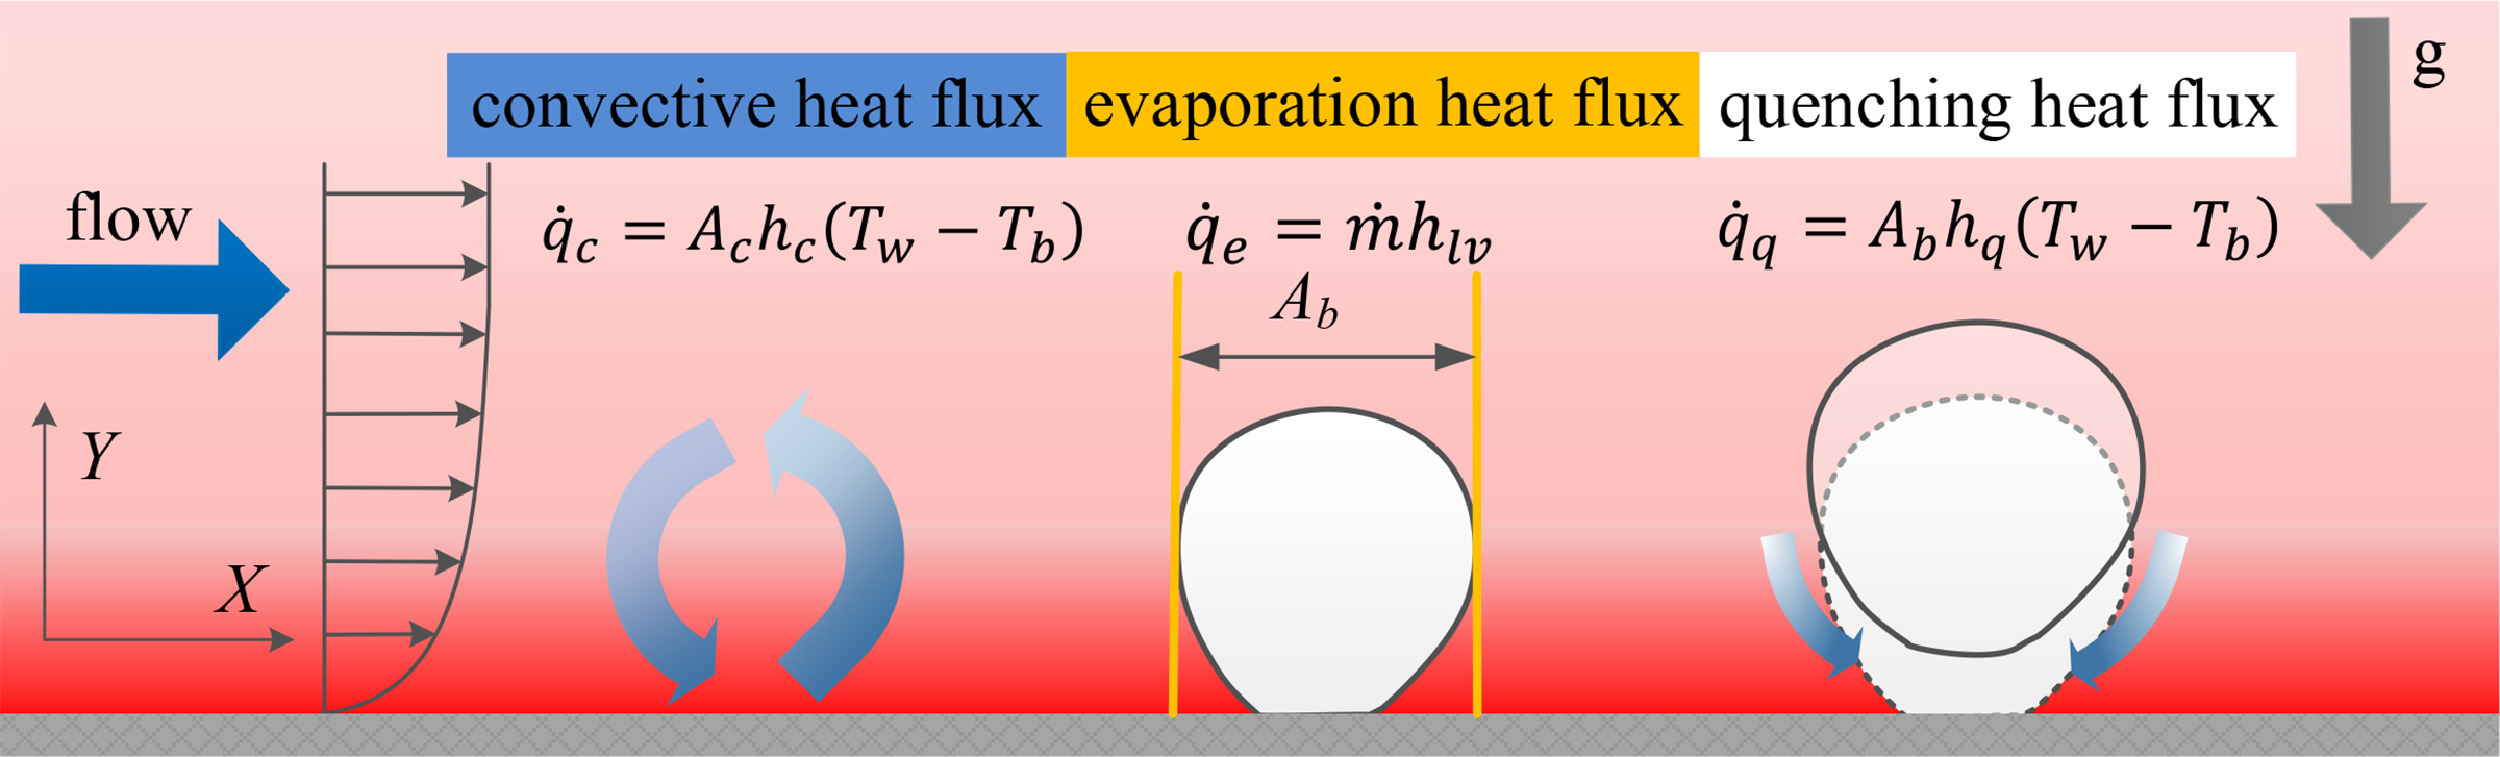
\includegraphics{Figure/Kurul.jpg}
    \caption{Depiction of the wall heat flux partitioning model for subcooled flow boiling from \textcite{ZHOU2021121295}.}
    \label{kurul}
\end{figure}
The model is implemented in :
\begin{lstlisting}[language=c++]
void Flux_parietal_Kurul_Podowski::set_param(Param& param)
\end{lstlisting}
The model implemented is :\\
1) Correction of single phase heat flux
\begin{itemize}
    \item[\small \textcolor{blue}{\ding{109}}]$\texttt{qpk}=\texttt{qpk}_{single\ phase}(1-A_{bub})$,
    \item[\small \textcolor{blue}{\ding{109}}]$\texttt{da\_qpk}=\texttt{da\_qpk}_{single\ phase}(1-A_{bub})$,
    \item[\small \textcolor{blue}{\ding{109}}]$\texttt{dp\_qpk}=\texttt{dp\_qpk}_{single\ phase}(1-A_{bub})$,
    \item[\small \textcolor{blue}{\ding{109}}]$\texttt{dv\_qpk}\texttt{=dv\_qpk}_{single\ phase}(1-A_{bub})$,
    \item[\small \textcolor{blue}{\ding{109}}]$\texttt{dTf\_qpk}=\texttt{dT_f\_qpk}_{single\ phase}(1-A_{bub})$,
    \item[\small \textcolor{blue}{\ding{109}}]$\texttt{dTp\_qpk}=\texttt{dTp\_qpk}_{single\ phase}(1-A_{bub})$.
\end{itemize}
2) Add partitioned heat flux
\begin{itemize}
    \item[\small \textcolor{blue}{\ding{109}}]$\texttt{dTp\_qpk} \pluseq -\texttt{qpk}_{single\ phase}(1-A_{bub})\frac{dA_{bub}}{dT_p}+\frac{dq_{quench}}{dT_p}$,
    \item[\small \textcolor{blue}{\ding{109}}]$\texttt{qpk}  \pluseq  q_{quench}$,
    \item[\small \textcolor{blue}{\ding{109}}]$\texttt{dTf\_qpk} \pluseq \frac{dq_{quench}}{dT_l}$,
    \item[\small \textcolor{blue}{\ding{109}}]$\texttt{qpi}  \pluseq  q_{evap}$,
    \item[\small \textcolor{blue}{\ding{109}}]$\texttt{dTp\_qpi} \pluseq \frac{dq_{evap}}{dT_p}$,
\end{itemize}
with
\begin{itemize}
    \item[\small \textcolor{blue}{\ding{109}}]Evaporation flux $q_{evap}=f_{dep}\frac{\pi d_b^3}{6}\rho_gL_{vap}N_{sites}$
    \item[\small \textcolor{blue}{\ding{109}}]Evaporation flux derivative regarding wall departure $\frac{dq_{evap}}{dT_p} =(\frac{df_{dep}}{dT_p}\frac{\pi d_b^3}{6}N_{sites}+f_{dep}\frac{3\pi d^2}{6}\frac{dd_b}{dT_p}N_{sites}+f_{dep}\frac{\pi d_b^3}{6}\frac{dN_{sites}}{dT_p})\rho_g L_{vap}$.
    \item[\small \textcolor{blue}{\ding{109}}]Quenching flux $q_{quench}=A_{bub}\sqrt{f_{dep}}\frac{2\lambda_l(T_p-T_l)}{\sqrt{\frac{\pi \lambda_l}{\rho_l Cp_l}}}$.
    \item[\small \textcolor{blue}{\ding{109}}]Quenching flux derivative regarding liquid temperature $\frac{d q_{quench}}{d T_l} =A_{bub}\sqrt{f_{dep}}\frac{-2\lambda_l}{\sqrt{\frac{\pi \lambda_l}{\rho_l Cp_l}}}$.
    \item[\small \textcolor{blue}{\ding{109}}]Quenching flux derivative regarding wall temperature $\frac{d q_{quench}}{d T_p} =\frac{d A_{bub}}{dT_p} \sqrt{f_{dep}}\frac{-2\lambda_l}{\sqrt{\frac{\pi \lambda_l}{\rho_l Cp_l}}}+A_{bub}\sqrt{f_{dep}}\frac{2\lambda_l}{\sqrt{\frac{\pi \lambda_l}{\rho_l Cp_l}}}-A_{bub}\frac{1}{2}\frac{df_{dep}}{dT_p}\frac{1}{\sqrt{f_{dep}}}\frac{2\lambda_l(T_p-T_l)}{\sqrt{\frac{\pi \lambda_l}{\rho_l Cp_l}}}$.
    \item[\small \textcolor{blue}{\ding{109}}]Number of evaporation sites $N_{sites}=(210\times{}(T_p-T_{sat}))^{1.8}$.
    \item[\small \textcolor{blue}{\ding{109}}]Number of evaporation sites $N_{sites}=(210\times{}(T_p-T_{sat}))^{1.8}$.
    \item[\small \textcolor{blue}{\ding{109}}]Number of evaporation sites derivative regarding wall temperature $\frac{d N_{sites}}{dT_p} =210\times 1.8(210.(T_p-T_{sat}))^{0.8}$.
    \item[\small \textcolor{blue}{\ding{109}}]Wall bubble diameter $d_b=0.0001(T_p-T_{sat})+0.0014$.
    \item[\small \textcolor{blue}{\ding{109}}]Wall bubble diameter derivative regrading wall temperature $\frac{dd_b}{dT_p}=0.0001$.
    \item[\small \textcolor{blue}{\ding{109}}]Wall bubble total area $A_{bub}=min(1.,\frac{\pi N_{sites}d_b^2}{4})$.
    \item[\small \textcolor{blue}{\ding{109}}]Wall bubble total area derivative regarding wall temperature  $\frac{dA_{bub}}{dT_p} =\frac{\pi d_b^2}{4}\frac{d N_{sites}}{dT_p} + \frac{\pi d_b N_{sites}}{2}\frac{d d_b}{dT_p}$, if $A_{bubbles}\neq 1.$, $0$, otherwise.
    \item[\small \textcolor{blue}{\ding{109}}]Departure frequency $f_dep=\sqrt{\frac{4}{3}\frac{9.81(\rho_l-\rho_g)}{\rho_l}}d_b^{-0.5}$.
    \item[\small \textcolor{blue}{\ding{109}}]Departure frequency derivative regarding wall temperature $\frac{d f_dep}{d T_p}=-0.5\frac{dd_b}{dT_p}d^{-1.5}\sqrt{\frac{4}{3}\frac{9.81(\rho_l-rho_g)}{\rho_l}}$

\end{itemize}

\subsection{Phase change}
The general expression of the phase change mass flux is :
\begin{equation}
    G(\alpha,p,T)
\end{equation}
It needs to be considered when there is a kinetic limit of gas for the phase change, for liquid metals, for example, but it does not apply to water.\\
The model is implemented in :
\begin{lstlisting}[language=c++]
void Changement_phase_base::set_param(Param& param)
\end{lstlisting}
The available input parameters are : 
\begin{lstlisting}[language=c++]
    double D_h;           // Hydraulic diameter
    double p;             // Pressure
    const double *alpha;  // Void fraction
    const double *T;      // Temperature
    const double *lambda; // Thermal conductivity
    const double *mu;     // Viscosity
    const double *rho;    // Density
    const double *Cp;     // Calorific capacity
    const double *Lvap;   // Latent heat
    const double *Tsat;   //Phase change saturated temperature
\end{lstlisting}
The phase change mass flux operator must fill dT_G, da_G, dp_G tabs and there derivative so that :
\begin{itemize}
    \item[\small \textcolor{blue}{\ding{109}}]$\texttt{G}$ mass flux
    \item[\small \textcolor{blue}{\ding{109}}] $\texttt{dT\_G}$ mass flux derivative regarding temperature   
    \item[\small \textcolor{blue}{\ding{109}}]$\texttt{dp\_G }$ mass flux derivative regarding pressure  
    \item[\small \textcolor{blue}{\ding{109}}]$\texttt{da\_G}$ mass flux derivative regarding void fraction  
\end{itemize}

\subsubsection{Silver Simpson}
The model is also described in  Silver and Simpson (1949, not found).

The model is implemented as:
\begin{lstlisting}[language=c++]
void Changement_phase_Silver_Simpson::set_param(Param& param)
{
  param.ajouter("lambda_e", &lambda_ec[0]); multiplicative factor for evaporation
  param.ajouter("lambda_c", &lambda_ec[1]); //  multiplicative factor for condensation
  param.ajouter("alpha_min", &alpha_min); // minimal void fraction to activate phase change
  param.ajouter("M", &M, Param::REQUIRED); // molar mass of steam
}
\end{lstlisting}
Default values : $\texttt{lambda\_ec[2]} = { 1, 1 }$, $\texttt{M} = -100.$, $\texttt{alpha\_min} = 0.1$.\\
The model implemented is :
\begin{align}
  &\texttt{dT\_G}_g = \texttt{fac} \times \texttt{var\_a} \times \frac{dT_{Psat}(T_g) - 0.5 \times \frac{Psat(T_g)}{T_g + T_0}}{\sqrt{T_g + T_0}}\\
  &\texttt{dT\_G}_l = \texttt{fac} \times \texttt{var\_a} \times 0.5 \times P \times (T_l + T_0)^{-1.5}\\
  &\texttt{da\_G}_g = \begin{cases} \texttt{fac} \times \texttt{var\_T} \times \texttt{var\_al}, if\  \alpha_g > \text{alpha\_min}, \\ 0,\ otherwise.\end{cases}\\
  &\texttt{da\_G}_l = \begin{cases} \texttt{fac} \times \texttt{var\_T} \times \texttt{var\_ak} \times 1.5 \times \sqrt{\alpha_l}, if\ \alpha_l > \texttt{alpha\_min},\\ 0,\ \text{otherwise}.
  \end{cases}\\
  &\texttt{dp\_G} = - \texttt{fac} \times \frac{\texttt{var\_a}}{\sqrt{T_l + T_0}}\\
  &\texttt{G} = \texttt{fac} \times\texttt{ var\_ak} \times \texttt{var\_al} \times \texttt{var\_T};
\end{align}
with
\begin{itemize}
    \item[\small \textcolor{blue}{\ding{109}}]$T_0 = 273.15$,
    \item[\small \textcolor{blue}{\ding{109}}]$\texttt{var\_ak}=\max(\alpha_g, \texttt{alpha\_min})$,
    \item[\small \textcolor{blue}{\ding{109}}]$\texttt{var\_al}=\parent{\max\parent{\alpha_l,\texttt{alpha\_min}}}^{1.5}$,
    \item[\small \textcolor{blue}{\ding{109}}]$\texttt{var\_a}=\texttt{var\_ak} \times \texttt{var\_al}$,
    \item[\small \textcolor{blue}{\ding{109}}]$\texttt{var\_T} = \frac{Psat(T_g)}{\sqrt{T_g + T_0}}  - \frac{P}{\sqrt{T_l + T_0}}$,
    \item[\small \textcolor{blue}{\ding{109}}]$\texttt{fac} = \lambda_{ec}[var_T < 0] \frac{4}{D_h}\sqrt{\frac{\texttt{M}}{2\texttt{M_{PI}}8.314}}$
\end{itemize}

\section{Analytical terms as source terms}\label{sec:analytical}
This section describes some analytical terms that are implemented as source terms in matrix.
%%
\subsection{Pressure term in energy equation}
This term arises from the averaging of the pressure work term due to the transport of internal energy instead of enthalpy. It represents the pressure work associated with changes in the distribution of void fraction. Its expression is :
\begin{equation}
    -P\parent{\frac{\partial \alpha_k}{\partial t}+\nabla \cdot (\alpha_k v_k)}
\end{equation}
It is implemented in: 
\begin{lstlisting}[language=c++]
void Source_Travail_pression_Elem_base::set_param(Param& param)
\end{lstlisting}
\subsection{Gravity}
Gravity is treated as a source term in \texttt{Pb_multiphase} and can't be as other problems from TrioCFD and TRUST. \\
The common way to add gravity is to add in the momentum equation a source. For example, with 2 phases :
\begin{lstlisting}[language=c++]
source_qdm Champ_Fonc_xyz dom 6 0 0 0 0 -9.81 -9.81
\end{lstlisting}
One must use \texttt{Gravite_Multiphase} to get gravity in momentum equation when using drift correlation.
The model is implemented as :
\begin{lstlisting}[language=c++]
void Gravite_Multiphase::set_param(Param& param)
{
  Noms noms(D), unites(D);
  noms[0] = "gravite";
  unites[0] = "m/s^2";
  Motcle typeChamp = "champ_elem" ;
  const Domaine_dis& z = ref_cast(Domaine_dis, pb.domaine_dis());
  dis.discretiser_champ(typeChamp, z.valeur(), scalaire, noms , unites, D, 0, gravite_);
}
\end{lstlisting}

\section{Injected sources of mass}\label{sec:injection}
It is necessary in order to simulate injectors of non-condensable bubbles, otherwise it boils.
\subsection{Injection of mass}
The model is implemented in:
\begin{lstlisting}[language=c++]
void Source_injection_masse_base::set_param(Param& param)
{
  Cerr << "Lecture du Champ de masse injectee" << finl;

  Champ_Don flux_masse_lu_;
  Motcle type;
  is >> type;

  flux_masse_lu_.typer(type);
  Champ_Don_base& ch_flux_masse_lu_ = ref_cast(Champ_Don_base,flux_masse_lu_.valeur());
  is >> ch_flux_masse_lu_;
  const int nb_comp = ch_flux_masse_lu_.nb_comp();

  equation().probleme().discretisation().discretiser_champ("champ_elem", equation().domaine_dis(), "pp", "1",nb_comp,0., flux_masse_);
  flux_masse_lu_->fixer_nb_comp(nb_comp);
  if (ch_flux_masse_lu_.le_nom()=="anonyme") ch_flux_masse_lu_.nommer("Flux_masse_injectee");

  for (int n = 0; n < nb_comp; n++) flux_masse_lu_->fixer_nom_compo(n, ch_flux_masse_lu_.le_nom() + (nb_comp > 1 ? Nom(n) :""));
  for (int n = 0; n < nb_comp; n++) flux_masse_->fixer_nom_compo(n, ch_flux_masse_lu_.le_nom() + (nb_comp > 1 ? Nom(n) :""));
  equation().discretisation().nommer_completer_champ_physique(equation().domaine_dis(),ch_flux_masse_lu_.le_nom(),"1/s",flux_masse_lu_,equation().probleme());
  equation().discretisation().nommer_completer_champ_physique(equation().domaine_dis(),ch_flux_masse_lu_.le_nom(),"1/s",flux_masse_,equation().probleme());
  flux_masse_.valeur().valeurs() = 0;
  flux_masse_.valeur().affecter(flux_masse_lu_);

  const Pb_Multiphase& pb = ref_cast(Pb_Multiphase, equation().probleme());
  int N = pb.nb_phases();
  if (N != flux_masse_.valeurs().line_size()) Process::exit(que_suis_je() + " : you must input as many fluxes as there are phases !!");

  return is;
}
\end{lstlisting}
In the mass equation:
\begin{equation}
    \texttt{secmem}  \pluseq  \rho_k f_{inj}
\end{equation}

\subsection{Momentum correction}
When a fluid flow is injected through a wall with zero momentum via a Neumann boundary condition on the mass equation, it is necessary to correct the momentum equation.

The model is implemented in:
\begin{lstlisting}[language=c++]
void Injection_QDM_nulle_PolyMAC_P0::set_param(Param& param)
{
  Param param(que_suis_je());
  param.ajouter("beta", &beta_);
  param.lire_avec_accolades_depuis(is);
}
\end{lstlisting}
Default values : $\texttt{beta\_} =1$.\\
Case 1: when bubbles are injected at the wall if not face from boundary
\begin{align}
    &\texttt{f\_a\_masse}=\rho_g U_{inj}\\
    &\texttt{f\_a}=\rho_g U_{inj}
\end{align}
corr-ajouter\_inj
\begin{align}
  &\texttt{secmem} \minuseq \texttt{surface}\times \texttt{f\_a\_masse}\times U^n\times \texttt{beta\_}\\
  &M_v \pluseq \texttt{surface}\times \texttt{f\_a\_masse}\times \texttt{beta\_}
\end{align}
Case 2: wall boiling if not face from boundary
\begin{align}
&\texttt{G}=\frac{q_p}{L_{vap}}\\
&\texttt{f\_a\_masse}  \minuseq \frac{\texttt{G}}{\texttt{surface}}\times \begin{cases} \frac{1}{\rho_g},\text{ if in gas,}\\-\frac{1}{\rho_l},\text{ if in liquid.} \end{cases}\\
&\texttt{f\_a}  \minuseq \frac{\texttt{G}}{\texttt{surface}}\times \begin{cases} 1,\text{ if in gas,}\\-1,\text{ if in liquid.}\end{cases}
\end{align}
corr-ajouter\_inj
\begin{align}
  &\texttt{secmem}  \minuseq  \texttt{surface} \times \texttt{f\_a\_masse}\times U^n\times \texttt{beta\_}\\
  &M_v \pluseq \texttt{surface}\times \texttt{f\_a\_masse}\times \texttt{beta\_}
\end{align}

%%%
\section{Equivalent diameter for dispersed phase\label{sec:diam-mgmt}}
\label{sec:IATE}
A fundamental aspect of modeling the interaction between liquid and gas phases lies in precisely predicting the concentration of interfaces. Some models rely on either the interfacial area concentration ($ai$) or an equivalent diameter ($Dsm$). In this context, the dispersed fluid is depicted as a collection of bubbles with diverse diameters, which essentially acts as a topological description for the fluid stage. This dispersed fluid is distinguished by two interlinked attributes: a distribution of bubble diameters and the concentration of interfaces. We can define the Sauter-Mean Diameter ($Dsm$) of the distribution ($f_d$) of sizes D as :
\begin{equation}
Dsm=\frac{\int f_dD^3 dD}{\int f_d D^2 dD}
\end{equation}
The relationship between the void fraction (\alpha) and the Sauter-Mean Diameter ($Dsm$)  hinges on calculating the area concentration per unit volume ($A_i=\pi D^2$). This relationship can be expressed as follows :
\begin{equation}
Dsm=\frac{\int f_dD^3 dD}{\int f_d D^2 dD}=6\frac{\int f_d V dv}{\int f_d A_i dV}=6\frac{\alpha}{ai}
\end{equation}
Finally, to have a correct representation of the dispersed phase, it is sufficient to impose an equivalent diameter, but it is also possible to add a transport equation for the interfacial area concentration.

%%
\subsection{User defined diameter}\label{Dsmuserdefine}

%
\subsubsection{Uniform diameter}\mbox{}
It is possible to simply impose a constant diameter at every point in space. The model is implemented in \texttt{Diametre_bulles_constant} :
\begin{lstlisting}[language=c++]
void Diametre_bulles_constant::set_param(Param& param)
{
  Param param(que_suis_je());
  param.ajouter("diametre", &d_bulle_, Param::REQUIRED);
  param.lire_avec_accolades_depuis(is);

  Pb_Multiphase& pb = ref_cast(Pb_Multiphase, pb_.valeur());
  int N = pb.nb_phases();
  const Discret_Thyd& dis=ref_cast(Discret_Thyd,pb.discretisation());
  Noms noms(N), unites(N);
  noms[0] = "diametre_bulles";
  unites[0] = "m";
  Motcle typeChamp = "champ_elem" ;
  const Domaine_dis& z = ref_cast(Domaine_dis, pb.domaine_dis());
  dis.discretiser_champ(typeChamp, z.valeur(), scalaire, noms , unites, N, 0, diametres_);

  champs_compris_.ajoute_champ(diametres_);

  for (int n = 0; n < pb.nb_phases(); n++) //recherche de n_l, n_g : phase {liquide,gaz}_continu en priorite
    if (pb.nom_phase(n).debute_par("liquide") && (n_l < 0 || pb.nom_phase(n).finit_par("continu")))  n_l = n;
  if (n_l < 0) Process::exit(que_suis_je() + " : liquid phase not found!");

  DoubleTab& tab_diametres = diametres_->valeurs();
  for (int i = 0 ; i < tab_diametres.dimension_tot(0) ; i++)
    for (int n = 0 ; n <N ; n++)
      if (n!=n_l) tab_diametres(i, n) = d_bulle_;

  return is;
}
\end{lstlisting}
Default value : $\texttt{d\_ bulle\_} =-100$.

%
\subsubsection{Non-uniform diameter}
It is possible to impose a user-defined diameter that varies spatially through the TRUST fields. The model is implemented in \texttt{Diametre_bulles_champ} :
\begin{lstlisting}[language=c++]
void Diametre_bulles_champ::set_param(Param& param)
{
  Champ_Don diametres_don_;
  is >> diametres_don_;

  Pb_Multiphase& pb = ref_cast(Pb_Multiphase, pb_.valeur());
  int N = pb.nb_phases();
  const Discret_Thyd& dis=ref_cast(Discret_Thyd,pb.discretisation());
  Noms noms(N), unites(N);
  noms[0] = "diametre_bulles";
  unites[0] = "m";
  Motcle typeChamp = "champ_elem" ;
  const Domaine_dis& z = ref_cast(Domaine_dis, pb.domaine_dis());
  dis.discretiser_champ(typeChamp, z.valeur(), scalaire, noms , unites, N, 0, diametres_);
  champs_compris_.ajoute_champ(diametres_);
  diametres_->affecter(diametres_don_.valeur());
  diametres_.valeurs().echange_espace_virtuel();
  return is;
}
\end{lstlisting}
Default value : $\texttt{d\_ bulle\_ }=-100$.

%%
\subsection{Interfacial area concentration with 1 group (incoming)}\label{Dsmu1grp}

%
\subsubsection{The general equation}
Two separated size-group methods are popular for the prediction of interfacial area concentration. One based on having an arbitrary number of groups to reproduce a distribution, referred as MUSIG or i-MUSIG \cite{Wang2005a,Das2010a,Liao2011} and the other reproducing the distribution thanks to the Mean Sauter diameter referred as IATE. The generalized Interfacial Area Transport Equation (IATE) developed by Kocamustafaogullari and Ishii \cite{Kocamustafaogullari,Kocamustafaogullari1994b}
The general expression for adiabatic flows with $\psi^{internal}_{j}$ a source term and $\psi^{intergroup}_j$ an intergroup term is then : \\

\begin{equation}
\frac{\partial a_{i}}{\partial t}+\underbrace{\nabla.(\mathbf{U} a_{i})}_{\colorbox{codebackground}{\color{codekeyword3} convection}}=\underbrace{\frac{2}{3}\frac{a_{i}}{\alpha}\frac{D\alpha}{Dt}}_{\colorbox{codebackground}{\color{codekeyword3} source\ of\ volume\ change}}+\underbrace{\color{myteal}\sum_j \psi^{intergroup}_{j}}_{\colorbox{codebackground}{\color{codekeyword3} intergroup\ sources}}+\underbrace{\color{myteal}\sum_j \psi^{internal}_{j}}_{\colorbox{codebackground}{\color{codekeyword3} intragroup sources}}.
\end{equation}
The terms in green need new modeling linked to coalescence and break-up.
Let's remind that :
\begin{equation}
 \frac{D\alpha\rho_g}{Dt}=\alpha\frac{d\rho_g}{dt}+\rho_g\frac{D\alpha}{Dt}=\Gamma_{transfer}+\Gamma_{nucleation}
 \end{equation}
Then we can substitute :
\begin{equation}
 \frac{D\alpha}{Dt}=\frac{1}{\rho_g}(\Gamma_{transfer}+\Gamma_{nucleation}-\alpha\frac{d\rho_g}{dt})
 \end{equation}
It gives the following equation :
\begin{equation}
\begin{aligned}
\frac{\partial a_{i}}{\partial t}+\underbrace{\nabla.(\mathbf{U} a_{i})}_{\colorbox{codebackground}{\color{codekeyword3} convection}}=\underbrace{-\frac{2}{3}\frac{a_{i}}{\rho_g}\frac{d\rho_g}{dt}}_{\colorbox{codebackground}{\color{codekeyword3} Density\ change}}+\underbrace{\frac{2}{3}\frac{a_{i}}{\alpha}\frac{\Gamma_{transfer}}{\rho_g}}_{\colorbox{codebackground}{\color{codekeyword3} Condensation}}+\underbrace{\frac{2}{3}\frac{a_{i}}{\alpha}\frac{\Gamma_{nucleation}}{\rho_g}}_{\colorbox{codebackground}{\color{codekeyword3} Nucleation}}&+ & \\\underbrace{\color{myteal} \sum_j \psi^{intergroup}_{j}}_{\colorbox{codebackground}{\color{codekeyword3} intergroup\ sources}}+\underbrace{\color{myteal} \sum_j \psi^{internal}_{j}}_{\colorbox{codebackground}{\color{codekeyword3} intragroup sources}}.
\end{aligned}
\end{equation}
The {\colorbox{codebackground}{\color{codekeyword3} Density\ change}} model is :
\begin{equation}
    -\frac{2}{3}\frac{a_{i}}{\rho_g}\frac{d\rho_g}{dt}
\end{equation}
The {\colorbox{codebackground}{\color{codekeyword3} Density\ change}} is implemented in \texttt{Variation_rho_Elem_PolyMAC_P0} :
\begin{lstlisting}[language=c++]
Void Variation_rho::set_param(Param& param)
\end{lstlisting}
It fills the following matrices :
\begin{align}
    &M_{ai} \minuseq  \frac{2}{3}\frac{1-\frac{\rho_g^{n-1}}{\rho_g^n}}{\Delta t}\\
    &M_{T} \minuseq  \frac{2}{3} \frac{a^n_i}{\Delta t} \frac{\rho_g^{n-1}}{(\rho_g^{n})^2}(-\texttt{dT\_rho})\\
    &M_{P} \minuseq  \frac{2}{3}\frac{a^n_i}{\Delta t} \frac{\rho_g^{n-1}}{(\rho_g^{n})^2}(-\texttt{dP\_rho})\\
    &\texttt{secmem} \pluseq  \frac{2}{3}a^n_i\frac{1-\frac{\rho_g^{n-1}}{\rho_g^n}}{\Delta t}
\end{align}
For example, the chain rule for the temperature gives :
\begin{equation}
    \frac{d(\frac{1}{\rho_g}\frac{d\rho_g}{dt})}{dT}=\frac{d\rho_g}{dT}\Bigg(\frac{d}{d\rho_g}(\frac{1}{\rho_g})\frac{d\rho_g}{dt}+\frac{1}{\rho_g}\frac{d}{d\rho_g}(\frac{d\rho_g}{dt}) \Bigg)=\frac{d\rho_g}{dT}\Bigg(-(\frac{1}{\rho_g^2})\frac{d\rho_g}{dt}+\frac{1}{\rho_g}\frac{d}{d\rho_g}(\frac{d\rho_g}{dt}) \Bigg)
\end{equation}
Regarding the discreet form, it gives :
\begin{equation}
   \frac{d\rho_g}{dT}\Bigg(-(\frac{1}{(\rho_g^n)^2})\frac{\rho_g^n-\rho_g^{n-1}}{\Delta t}+\frac{1}{\rho_g^n\Delta t}\Bigg)=\frac{1}{\Delta t}\frac{d\rho_g}{dT}\Bigg(\frac{\rho_g^{n-1}}{(\rho_g^n)^2}\Bigg)
\end{equation}
The {\colorbox{codebackground}{\color{codekeyword3} Condensation}} model is :
\begin{equation}
    \frac{2}{3}\frac{a_i}{\alpha \rho_g} G,
\end{equation}
with G given by a correlation.\\
The {\colorbox{codebackground}{\color{codekeyword3} Condensation}} term is implemented in \texttt{Source_Flux_interfacial_base} as :
\begin{equation}
    \texttt{secmem}  \pluseq  \frac{2}{3}\frac{a_i^n}{\alpha^n\rho_g^n} G^n
\end{equation}
If the condensation is not making the phase evanescent then : 
\begin{align}
    &M_\alpha  \minuseq  \frac{-2}{3}\frac{a_i^n}{(\alpha^n)^2}\rho_g^n G^n\\
    &M_T  \minuseq  \frac{-2}{3}\frac{a_i^n}{\alpha^n(\rho_g^n)^2} G^n \frac{d\rho_l}{dT}+\frac{2}{3}\frac{a_i^n}{\alpha^n\rho_g} \frac{dG}{dT}\\
    &M_P  \minuseq  \frac{-2}{3}\frac{a_i^n}{\alpha^n(\rho_g^n)^2} G^n \frac{d\rho_g}{dP}+\frac{2}{3}\frac{a_i^n}{\alpha^n\rho_g} \frac{dG}{dP}\\
    &M_{a_i}  \minuseq  \frac{2}{3}\frac{1}{\alpha^n\rho_g^n} G^n
\end{align}

For the other source terms, refer to the models.

%
\subsubsection{The Yao Morel model}
The model is described in \textcite{YAO2004307}.

The equation is: 
\begin{equation}
\frac{\partial a_{i}}{\partial t}+\underbrace{\nabla.(\mathbf{U} a_{i})}_{\colorbox{codebackground}{\color{codekeyword3} convection}}=\underbrace{\frac{2}{3}\frac{a_{i}}{\alpha}(\frac{\Gamma_{condensation}}{\rho_g}-\frac{\alpha_g}{\rho_g} \frac{d \rho_g}{d t})}_{\colorbox{codebackground}{\color{codekeyword3} source\ of\ volume\ change}}+\underbrace{\pi d_{dep}^2\Phi_N}_{\colorbox{codebackground}{\color{codekeyword3} Nucleation}}+\underbrace{\frac{36\pi}{3}(\frac{\alpha}{a_i})^2{\color{myteal}\Phi_{coal}}}_{\colorbox{codebackground}{\color{codekeyword3} Coalescence}}+\underbrace{\frac{36\pi}{3}(\frac{\alpha}{a_i})^2{\color{myteal}\Phi_{breakup}}}_{\colorbox{codebackground}{\color{codekeyword3}  Break-up}}.
\end{equation}
The {\colorbox{codebackground}{\color{codekeyword3} Coalescence}} model is : 
\begin{equation}
\begin{aligned}
		\frac{36\pi}{3}(\frac{\alpha}{a_i})^2\Phi_{Coal} =- \frac{36\pi}{3}(\frac{\alpha}{a_i})^2 (\varepsilon d_b)^{1/3} \cdot \frac{\alpha^2}{d_b^4} \cdot K_{c1} \cdot \frac{1}{g(\alpha) + K_{c2}\alpha \sqrt{We/We_{cr}}} \cdot \text{exp}\left(-K_{c3} \sqrt{\frac{We}{We_{cr}}}\right)& & \\ = {\color{mydarkorchid} \frac{\pi}{3\times 6^{5/3}}\alpha^{1/3}a_i^{5/3}\varepsilon^{1/3}} \cdot {\color{myslateblue} K_{c1} \frac{-1}{g(\alpha) + K_{c2}\alpha \sqrt{We/We_{cr}}} \cdot \text{exp}\left(-K_{c3} \sqrt{\frac{We}{We_{cr}}}\right)},
\end{aligned}
\end{equation}
with $K_{c1} = 2.86$, $K_{c2} = 1.922$, $K_{c3} = 1.017$, $We_{cr} = 1.24$, $g(\alpha) = \frac{\alpha_\text{max}^{1/3}-\alpha^{1/3}}{\alpha_\text{max}^{1/3}}$, $\alpha_\text{max} = \frac{\pi}{6}$.\\
The {\colorbox{codebackground}{\color{codekeyword3} Coalescence}} model is implemented as $\frac{36\pi}{3}(\frac{\alpha}{a_i})^2\Phi_{Coal}={\color{mydarkorchid}f_1(\alpha,ai,k,\varepsilon)}{\color{myslateblue} f_2(\alpha,ai,k,\varepsilon)}$ so that for the sake of simplicity $d({\color{mydarkorchid}f_1}{\color{myslateblue} f_2})={\color{myslateblue} f_2}d{\color{mydarkorchid} f_1}$  in {\color{mydarkorchid} Coalescence_bulles_1groupe_PolyMAC_P0} : 
\begin{lstlisting}[language=c++]
void Coalescence_bulles_1groupe_PolyMAC_P0::set_param(Param& param)
{
  Param param(que_suis_je());
  param.ajouter("beta_k", &beta_k_);
}
\end{lstlisting}
and {\color{myslateblue} Coalescence_bulles_1groupe_Yao_Morel}:
\begin{lstlisting}[language=c++]
void Coalescence_bulles_1groupe_Yao_Morel::set_param(Param& param)
\end{lstlisting}
Default values : $\texttt{beta\_k\_} = 0.09$, $\texttt{Kc1} = 2.86$, $\texttt{Kc2} = 1.922$, $\texttt{Kc3} = 1.017$,
$\texttt{alpha\_max\_1\_3} = (\frac{\pi}{6})^{1/3}$, $\texttt{We\_cr} = 1.24$.\\
{\color{red} Warning} : The following part describes the matrix filling for the $k-\varepsilon$ model, as an example, but it is currently not implemented since only the $k-\tau$ and $k-\omega$ models are available and are the only ones implemented for the source terms.\\
For the $k-\varepsilon$ model : 
\begin{align}
    &M_{\alpha} \minuseq \frac{\pi}{3\times 6^{5/3}}\frac{1}{3}(\alpha^n)^{-2/3}(a_i^n)^{5/3}(\varepsilon^n)^{1/3} {\color{myslateblue} f_2^n}\\
    &M_{a_i} \minuseq \frac{\pi}{3\times 6^{5/3}}\frac{5}{3}(\alpha^n)^{1/3}(a_i^n)^{2/3}(\varepsilon^n)^{1/3} {\color{myslateblue} f_2^n}\\
    &M_{k}=0\\
    &M_{\varepsilon} \minuseq \frac{\pi}{3\times 6^{5/3}}\frac{1}{3}(\alpha^n)^{-2/3}(a_i^n)^{5/3}(\varepsilon^n)^{-2/3} {\color{myslateblue} f_2^n}\\
    &\text{secmem} \pluseq \frac{\pi}{3\times 6^{5/3}}(\alpha^n)^{1/3}(a_i^n)^{5/3}(\varepsilon^n)^{1/3} {\color{myslateblue} f_2^n}
\end{align}
If the $k-\tau$ turbulence model is used, 
\begin{equation}
\varepsilon = \frac{k^2}{\text{max}(k\tau, \texttt{visc\_turb.limiteur()} \nu_l)}\times \texttt{beta\_k\_}.
\end{equation}
If the $k-\omega$ turbulence model is used, 
\begin{equation}
\varepsilon = k \times \omega \times\texttt{ beta\_k\_}.
\end{equation}
The {\colorbox{codebackground}{\color{codekeyword3}  Break-up}} model is : 
\begin{equation}
\begin{aligned}
		\frac{36\pi}{3}\parent{\frac{\alpha}{a_i}}^2\Phi_{\text{breakup}} =- \frac{36\pi}{3}\parent{\frac{\alpha}{a_i}}^2 \parent{\varepsilon d_b}^{1/3} \cdot \frac{\alpha(1-\alpha)}{d_b^4} \cdot K_{b1} \cdot \frac{1}{1 + K_{b2}\alpha_l \sqrt{We/We_{cr}}} \cdot \text{exp}\left(- \frac{We}{We_{cr}}\right)& & \\ = {\color{mydarkorchid} \frac{\pi}{3\times 6^{5/3}}\alpha^{-2/3}(1-\alpha)a_i^{5/3}\varepsilon^{1/3}} \cdot {\color{myslateblue} K_{b1} \cdot \frac{1}{1 + K_{b2}(1-\alpha) \sqrt{We/We_{cr}}} \cdot \text{exp}\left(- \frac{We}{We_{cr}}\right)},
\end{aligned}
\end{equation}
with $K_{b1} = 1.6$, $K_{b2} = 0.42$, $We_{cr} = 1.24$.

The {\colorbox{codebackground}{\color{codekeyword3}  Break-up}} model is implemented as $\frac{36\pi}{3}\parent{\frac{\alpha}{a_i}}^2\Phi_{\text{breakup}}={\color{mydarkorchid}f_1(\alpha,ai,k,\varepsilon)}{\color{myslateblue} f_2(\alpha,ai,k,\varepsilon)}$ so that for the sake of simplicity $d({\color{mydarkorchid}f_1}{\color{myslateblue} f_2})={\color{myslateblue} f_2}d{\color{mydarkorchid} f_1}$  in {\color{mydarkorchid} Rupture_bulles_1groupe_PolyMAC_P0} : 
\begin{lstlisting}[language=c++]
void Rupture_bulles_1groupe_PolyMAC_P0::set_param(Param& param)
{
  Param param(que_suis_je());
  param.ajouter("beta_k", &beta_k_);
}
\end{lstlisting}
and {\color{myslateblue} Rupture_bulles_1groupe_Yao_Morel}:
\begin{lstlisting}[language=c++]
void Rupture_bulles_1groupe_Yao_Morel::set_param(Param& param)
\end{lstlisting}
Default values: $\texttt{beta\_k\_} = 0.09$, $\texttt{Kb1} = 1.6$, $\texttt{Kb2} = 0.42$, $\texttt{We\_cr} = 1.24$.\\
{\color{red} Warning} : The following part describes the matrix filling for the $k-\varepsilon$ model, as an example, but it is currently not implemented since only the $k-\tau$ and $k-\omega$ models are available and are the only ones implemented for the source terms.\\
For the $k-\varepsilon$ model : 
\begin{align}
    &M_{\alpha} \minuseq \frac{\pi}{3\times 6^{5/3}}\frac{-2}{3}(\alpha^n)^{-5/3}\alpha_l^n(a_i^n)^{5/3}(\varepsilon^n)^{1/3} {\color{myslateblue} f_2^n}\\
    &M_{\alpha_l} \minuseq \frac{\pi}{3\times 6^{5/3}}(\alpha^n)^{-2/3}(a_i^n)^{5/3}(\varepsilon^n)^{1/3} {\color{myslateblue} f_2^n}\\
    &M_{a_i} \minuseq \frac{\pi}{3\times 6^{5/3}}\frac{5}{3}(\alpha^n)^{1/3}\alpha_l^n(a_i^n)^{2/3}(\varepsilon^n)^{1/3} {\color{myslateblue} f_2^n}\\
    &M_{k}=0\\
    &M_{\varepsilon} \minuseq \frac{\pi}{3\times 6^{5/3}}\frac{1}{3}(\alpha^n)^{-2/3}\alpha_l^n(a_i^n)^{5/3}(\varepsilon^n)^{-2/3} {\color{myslateblue} f_2^n}\\
    &\text{secmem}  \pluseq  \frac{\pi}{3\times 6^{5/3}}\frac{1}{3}(\alpha^n)^{-2/3}\alpha_l^n(a_i^n)^{5/3}(\varepsilon^n)^{-2/3} {\color{myslateblue} f_2^n}\\
\end{align}
If the $k-\tau$ turbulence model is used, 
\begin{equation}
\varepsilon=\frac{k^2}{\text{max}(k\tau,\ \texttt{visc_turb.limiteur()} \nu_l)}\times beta\_ k \_.
\end{equation}
If the $k-\omega$ turbulence model is used
\begin{equation}
\varepsilon=k\times \omega\times beta\_ k \_.
\end{equation}
The {\colorbox{codebackground}{\color{codekeyword3}  Nucleation}} model is : 
\begin{equation}
		\pi d_{dep}^2\Phi_N = \pi d_{dep}^2\frac{\Phi_{e}}{L_{\text{vap}} \rho_g \frac{\pi}{6}d_\text{dep}^3}=6\frac{\Phi_{\text{nucleation}}}{\text{max}(d_{\text{nuc}},10^{-8})\rho_g L_{\text{vap}}}
\end{equation}
with $\Phi_{e}$ wall heat transfer.

The {\colorbox{codebackground}{\color{codekeyword3}  Nucleation}} model is implemented in Nucleation_paroi_PolyMAC_P0: 
\begin{lstlisting}[language=c++]
void Nucleation_paroi_PolyMAC_P0::set_param(Param& param)
\end{lstlisting}
This terms injected only on boundary elements and is fully explicit: 
\begin{equation}
    \texttt{secmem} \pluseq 6\frac{\Phi_{\text{nucleation}}^n}{\text{max}(d_{\text{nuc}}^n,10^{-8})\rho_g^n L_{\text{vap}}^n}
\end{equation}

%%
\subsection{Interfacial area concentration with 2 groups (incoming)}

%
\subsubsection{The equations}
A particular case of the solution can be obtained if we consider two groups of bubbles. For example, experimentally a limit can be observed between quasi-spherical and distorted bubbles. Then we can separate the distribution of those groups into 2 distinct distributions on either side of the critical diameter $Dsmc=4\sqrt{\tfrac{\sigma}{g(\rho_l-\rho_g)}}$, with $\sigma$ the surface tension, $g$ gravity and $\rho_g$ and $\rho_l$ respectively the densities of the gas and the liquid. For the first group we get :
\begin{equation}
\begin{aligned}
\frac{\partial a_{i1}}{\partial t}+\underbrace{\nabla\parent{a_{i1}\mathbf{U}_{g1}}}_{\colorbox{codebackground}{\color{codekeyword3} convection}}=&\underbrace{\frac{2}{3}\frac{a_{i1}}{\alpha_{g1}}\parent{-\frac{\alpha_{g1}}{\rho_g}\frac{d \rho_g}{dt}}}_{\colorbox{codebackground}{\color{codekeyword3} Density\ change}}-\underbrace{\chi_d\parent{\frac{D_{smc}}{D_{sm1}}}^2\frac{a_{i1}}{\alpha_{g1}}\parent{-\frac{\alpha_{g1}}{\rho_g}\frac{d \rho_g}{dt}}}_{\colorbox{codebackground}{\color{codekeyword3} Density\ sliding}}  \\
&+\underbrace{\frac{2}{3}\frac{a_{i1}}{\alpha_{g1}}\parent{\frac{\color{myteal}\Gamma_{g1}}{\rho_g}}}_{\colorbox{codebackground}{\color{codekeyword3} Mass\ transfer}}-\underbrace{\chi_d\parent{\frac{D_{smc}}{D_{sm1}}}^2\frac{a_{i1}}{\alpha_{g1}}\parent{\frac{\color{myteal}\Gamma_{g1}}{\rho_g}}}_{\colorbox{codebackground}{\color{codekeyword3} Mass\ transfer\ sliding}} \\
&+\underbrace{\color{myteal}\sum_j \psi^{\text{intergroup}}_{1j}}_{\colorbox{codebackground}{\color{codekeyword3} intergroup\ sources}}+\underbrace{\color{myteal}\sum_j \psi^{\text{internal}}_{1j}}_{\colorbox{codebackground}{\color{codekeyword3} intragroup sources}}.
\end{aligned}
\end{equation}
For the second group, we get:
\begin{equation}
\begin{aligned}
\frac{\partial a_{i2}}{\partial t}+\underbrace{\nabla\parent{a_{i2}\mathbf{U}_{g2}}}_{\colorbox{codebackground}{\color{codekeyword3} convection}}=\underbrace{\frac{2}{3}\frac{a_{i2}}{\alpha_{g2}}\parent{-\frac{\alpha_{g2}}{\rho_g}\frac{d \rho_g}{dt}}}_{\colorbox{codebackground}{\color{codekeyword3} Density\ change}}+\underbrace{\chi_d\parent{\frac{D_{smc}}{D_{sm1}}}^2\frac{a_{i1}}{\alpha_{g1}}\parent{-\frac{\alpha_{g1}}{\rho_g}\frac{d \rho_g}{dt}}}_{\colorbox{codebackground}{\color{codekeyword3} Density\ sliding}}&+ & \\
\underbrace{\frac{2}{3}\frac{a_{i2}}{\alpha_{g2}}\parent{\frac{\color{myteal}\Gamma_{g2}}{\rho_g}}}_{\colorbox{codebackground}{\color{codekeyword3} Mass\ transfer}} +\underbrace{\chi_d\parent{\frac{D_{smc}}{D_{sm1}}}^2\frac{a_{i1}}{\alpha_{g1}}\parent{\frac{\color{myteal}\Gamma_{g1}}{\rho_g} }}_{\colorbox{codebackground}{\color{codekeyword3} Mass\ transfer\ sliding}} +& \\ 
\underbrace{\color{myteal}\sum_j \psi^{\text{intergroup}}_{2j}}_{\colorbox{codebackground}{\color{codekeyword3} intergroup\ sources}}+\underbrace{\color{myteal}\sum_j \psi^{\text{internal}}_{2j}}_{\colorbox{codebackground}{\color{codekeyword3} intragroup sources}}.
\end{aligned}
\end{equation}
The different mass transfer are:
\begin{equation}
\begin{aligned}
\Gamma_{g1}=\underbrace{-\frac{\rho_g}{1+\chi_d \parent{\frac{Dsmc}{Dsm1}}^3}{\color{myteal}\sum_j \eta^{inter}_j}}_{\colorbox{codebackground}{\color{codekeyword3} Intergroup}}+ \underbrace{\frac{\chi_d\parent{\frac{D_{smc}}{D_{sm1}}}^3}{1+\chi_d \parent{\frac{Dsmc}{Dsm1}}^3}\alpha_{g1}\parent{\frac{d\rho_{g}}{dt}}}_{\colorbox{codebackground}{\color{codekeyword3} Density\ group\ shift}}&+& \\
\underbrace{\frac{1}{1+\chi_d \parent{\frac{Dsmc}{Dsm1}}^3}\Gamma_{\text{condensation g1}}}_{\colorbox{codebackground}{\color{codekeyword3} Condensation}}+\underbrace{\frac{\chi_d\parent{\frac{D_{smc}}{D_{sm1}}}^3}{1+\chi_d \parent{\frac{Dsmc}{Dsm1}}^3}\Gamma_{\text{Nucleation g1}}}_{\colorbox{codebackground}{\color{codekeyword3} Nucleation}}.
\end{aligned}
\end{equation}
\begin{equation}
\begin{aligned}
\Gamma_{g2}=\underbrace{\frac{\rho_g}{1+\chi_d \parent{\frac{Dsmc}{Dsm1}}^3}{\color{myteal}\sum_j \eta^{inter}_j}}_{\colorbox{codebackground}{\color{codekeyword3} Intergroup}}- \underbrace{\frac{\chi_d\parent{\frac{D_{smc}}{D_{sm1}}}^3}{1+\chi_d \parent{\frac{Dsmc}{Dsm1}}^3}\alpha_{g1}\parent{\frac{d\rho_{g}}{dt}}}_{\colorbox{codebackground}{\color{codekeyword3} Density\ group\ shift}}&+& \\
\underbrace{\Gamma_{\text{condensation\ g2}}+\frac{\chi_d \parent{\frac{Dsmc}{Dsm1}}^3}{1+\chi_d \parent{\frac{Dsmc}{Dsm1}}^3}\Gamma_{\text{condensation g1}}}_{\colorbox{codebackground}{\color{codekeyword3} Condensation}}-\underbrace{\frac{\chi_d\parent{\frac{D_{smc}}{D_{sm1}}}^3}{1+\chi_d \parent{\frac{Dsmc}{Dsm1}}^3}\Gamma_{\text{Nucleation g1}}}_{\colorbox{codebackground}{\color{codekeyword3} Nucleation}}.
\end{aligned}
\end{equation}
$\chi_d$ is equal to $1$ for a uniform distribution profile. Indeed, because there is no prior determination of the form of the solution of the distribution, the easiest from to consider is a uniform distribution.
During the averaging process proposed in \cite{Kataoka2012} , two new terms emerged from the instantaneous equation: a diffusion term and a lift term. For example, the diffusion term can be implemented as: 
\begin{equation}
K\sqrt{u^{\prime 2}}D_{sm}\nabla a_i=K\sqrt{\frac{2k}{3}} D_{sm}\nabla a_i,
\end{equation}
with $K$ a constant equal to $1/3$. However, it is essential to note that these terms have not yet been fully validated in various configurations \cite{Rassame2023}. For the implementation in the code, we must rewrite it to get rid of $D_{sm}$. For the first group we have:
\begin{equation}
\begin{aligned}
\frac{\partial a_{i1}}{\partial t}+\underbrace{\nabla\parent{a_{i1}\mathbf{U}_{g1}}}_{\colorbox{codebackground}{\color{codekeyword3} convection}}=\underbrace{\frac{2}{3}\frac{a_{i1}}{\alpha_{g1}}\parent{-\frac{\alpha_{g1}}{\rho_g}\frac{d \rho_g}{dt}}}_{\colorbox{codebackground}{\color{codekeyword3} Density\ change}}-\underbrace{\frac{\chi_d}{36}D_{smc}^2\parent{\frac{a_{i1}}{\alpha_{g1}}}^3\parent{-\frac{\alpha_{g1}}{\rho_g}\frac{d \rho_g}{dt}}}_{\colorbox{codebackground}{\color{codekeyword3} Density\ sliding}} &+& \\\underbrace{\frac{2}{3}\frac{a_{i1}}{\alpha_{g1}}\parent{\frac{\color{myteal}\Gamma_{g1}}{\rho_g}}}_{\colorbox{codebackground}{\color{codekeyword3} Mass\ transfer}}-\underbrace{\frac{\chi_d}{36}D_{smc}^2\parent{\frac{a_{i1}}{\alpha_{g1}}}^3\parent{\frac{\color{myteal}\Gamma_{g1}}{\rho_g}}}_{\colorbox{codebackground}{\color{codekeyword3} Mass\ transfer\ sliding}}+& \\\underbrace{\color{myteal}\sum_j \psi^{intergroup}_{1j}}_{\colorbox{codebackground}{\color{codekeyword3} intergroup\ sources}}+\underbrace{\color{myteal}\sum_j \psi^{internal}_{1j}}_{\colorbox{codebackground}{\color{codekeyword3} intragroup sources}}.
\end{aligned}
\end{equation}
For the second group, we obtain:
\begin{equation}
\begin{aligned}
\frac{\partial a_{i2}}{\partial t}+\underbrace{\nabla\parent{a_{i2}\mathbf{U}_{g2}}}_{\colorbox{codebackground}{\color{codekeyword3} convection}}=\underbrace{\frac{2}{3}\frac{a_{i2}}{\alpha_{g2}}\parent{-\frac{\alpha_{g2}}{\rho_g}\frac{d \rho_g}{dt}}}_{\colorbox{codebackground}{\color{codekeyword3} Density\ change}}+\underbrace{\frac{\chi_d}{36}D_{smc}^2\parent{\frac{a_{i1}}{\alpha_{g1}}}^3\parent{-\frac{\alpha_{g1}}{\rho_g}\frac{d \rho_g}{dt}}}_{\colorbox{codebackground}{\color{codekeyword3} Density\ sliding}}&+ & \\
\underbrace{\frac{2}{3}\frac{a_{i2}}{\alpha_{g2}}\parent{\frac{\color{myteal}\Gamma_{g2}}{\rho_g}}}_{\colorbox{codebackground}{\color{codekeyword3} Mass\ transfer}} +\underbrace{\frac{\chi_d}{36}D_{smc}^2\parent{\frac{a_{i1}}{\alpha_{g1}}}^3\parent{\frac{\color{myteal}\Gamma_{g1}}{\rho_g} }}_{\colorbox{codebackground}{\color{codekeyword3} Mass\ transfer\ sliding}} +& \\ 
\underbrace{\color{myteal}\sum_j \psi^{\text{intergroup}}_{2j}}_{\colorbox{codebackground}{\color{codekeyword3} intergroup\ sources}} + \underbrace{\color{myteal}\sum_j \psi^{\text{internal}}_{2j}}_{\colorbox{codebackground}{\color{codekeyword3} intragroup sources}}.
\end{aligned}
\end{equation}
The different mass transfer are:
\begin{equation}
\begin{aligned}
\Gamma_{g1} = \underbrace{-\frac{\rho_g}{1+\frac{\chi_d}{216}Dsmc^3\parent{\frac{a_{i1}}{\alpha_{g1}}}^3}{\color{myteal}\sum_j \eta^{inter}_j}}_{\colorbox{codebackground}{\color{codekeyword3} Intergroup}}+ \underbrace{\frac{\frac{\chi_d}{216}Dsmc^3\parent{\frac{a_{i1}}{\alpha_{g1}}}^3}{1+\frac{\chi_d}{216}Dsmc^3\parent{\frac{a_{i1}}{\alpha_{g1}}}^3}\alpha_{g1}\parent{\frac{d\rho_{g}}{dt}}}_{\colorbox{codebackground}{\color{codekeyword3} Density\ group\ shift}}&+& \\
\underbrace{\frac{1}{1+\frac{\chi_d}{216}Dsmc^3\parent{\frac{a_{i1}}{\alpha_{g1}}}^3}\Gamma_{\text{condensation g1}}}_{\colorbox{codebackground}{\color{codekeyword3} Condensation}}+\underbrace{\frac{\frac{\chi_d}{216}Dsmc^3\parent{\frac{a_{i1}}{\alpha_{g1}}}^3}{1+\frac{\chi_d}{216}Dsmc^3\parent{\frac{a_{i1}}{\alpha_{g1}}}^3}\Gamma_{\text{Nucleation g1}}}_{\colorbox{codebackground}{\color{codekeyword3} Nucleation}}.
\end{aligned}
\end{equation}
\begin{equation}
\begin{aligned}
\Gamma_{g2}=\underbrace{\frac{\rho_g}{1+\frac{\chi_d}{216}Dsmc^3(\frac{a_{i1}}{\alpha_{g1}})^3}{\color{myteal}\sum_j \eta^{inter}_j}}_{\colorbox{codebackground}{\color{codekeyword3} Intergroup}}- \underbrace{\frac{\frac{\chi_d}{216}Dsmc^3(\frac{a_{i1}}{\alpha_{g1}})^3}{1+\frac{\chi_d}{216}Dsmc^3(\frac{a_{i1}}{\alpha_{g1}})^3}\alpha_{g1}\parent{\frac{d\rho_{g}}{dt}}}_{\colorbox{codebackground}{\color{codekeyword3} Density\ group\ shift}}&+& \\
\underbrace{\Gamma_{\text{condensation g2}} + \frac{\frac{\chi_d}{216}Dsmc^3(\frac{a_{i1}}{\alpha_{g1}})^3}{1+\frac{\chi_d}{216}Dsmc^3(\frac{a_{i1}}{\alpha_{g1}})^3}\Gamma_{\text{condensation g1}}}_{\colorbox{codebackground}{\color{codekeyword3} Condensation}}-\underbrace{\frac{\frac{\chi_d}{216}Dsmc^3(\frac{a_{i1}}{\alpha_{g1}})^3}{1+\frac{\chi_d}{216}Dsmc^3(\frac{a_{i1}}{\alpha_{g1}})^3}\Gamma_{\text{Nucleation g1}}}_{\colorbox{codebackground}{\color{codekeyword3} Nucleation}}.
\end{aligned}
\end{equation}

%
\subsubsection{The source terms}
All source term models are based on five categories of mechanism: the Random Collisions (RC), the Wake Entrainment (WE), the Turbulent Impacts (TI), the Shearing-off (SO) and the Surface Instability (SI) (see Figure \ref{bulles}). The RC is a bubble coalescence phenomenon where $2$ bubbles collide and merge because of a turbulent eddy of comparable size. The WE happens when one smaller bubble is in the wake of a bigger one, accelerates and collides it. The TI is due to turbulent eddies that break-up bubbles. The SO is a break-up phenomenon that source from the shearing-off of cap bubbles. The SI is due to the break-up of large bubbles due to their surface instability.\\
The number of processes and the dimensionless coefficient can strongly differ from one model to another : 
\begin{itemize}
\item[\small \textcolor{blue}{\ding{109}}] The \textcite{SUN2} model was developed for a $2$ group configuration with a $200 \times  10$ $mm^2$ confined rectangular channel data. The effect of the wall is then very significant. It was performed for liquid superficial velocity between $0.32$ and $2.84$ m/s and gas velocity between $0.39$ and $2.01$ m/s. It deals with cap-bubbly and churn-turbulent flows.\\
\item[\small \textcolor{blue}{\ding{109}}] The \textcite{Smith1} model was developed for a $2$ group configuration with $0.102$ mm and $0.152$ mm diameter pipes. It deals with bubbly, cap-bubbly and churn-turbulent flows. \\
\item[\small \textcolor{blue}{\ding{109}}] The \textcite{Schlegel1} model was developed for a $2$ group configuration with large diameter channels. It deals with bubbly and cap-bubbly flows. Several constitutive relations and correlations were used to tune this model.\\
\item[\small \textcolor{blue}{\ding{109}}] The \textcite{Fu2002} model was developed for a $2$ group configuration for small round pipe.\\
\item[\small \textcolor{blue}{\ding{109}}] \textcite{Dave2016a} proposed new Smith coefficient based on optimization with genetic algorithm on all TOPFLOW DN200 (pipe $195.3$ mm).
\end{itemize}
\begin{figure}[!ht]
    \centering
    \includegraphics[scale=1]{Figure/bulles2.png}
    \caption{Representation of 2 group bubble mechanisms.}
    \label{bulles}
\end{figure}
The coefficients of the previous models are summarized in Table \ref{coeff2grp}.
\begin{table}[!ht]
\begin{center}
\begin{tabular}{c c c c c c } 
\toprule
Coefficient & Sun \cite{SUN2} & Smith \cite{Smith1} & Schlegel \cite{Schlegel1} & Fu \cite{Fu2002} & Dave \cite{Dave2016a}\\ 
\midrule
\rowcolor[gray]{0.9} $C^{(1)}_{RC}$ & $0.005$ &$0.01$ & $0.01$ & $0.0041$ & $0.26$ \\  
 $C^{(12,2)}_{RC}$ & $0.005$ & $0.01$ & $0.05$ & $0.005$ & $0.41$ \\ 
 \rowcolor[gray]{0.9} $C^{(2)}_{RC}$ & $0.005$ & $0.01$ & $0.01$ & $0.005$ & $1.00$ \\  
 $C_{RC0}$ & $3.0$ & $3.0$ & $3.0$ & $3.0$ & $3.0$ \\ 
 \rowcolor[gray]{0.9} $C_{RC1}$ & $3.0$ & $3.0$ & $3.0$  & $3.0$ & $3.0$ \\  
 $\alpha_{g1,max}$ & $0.62$ & $0.62$ & $0.62$& $0.75$ & $0.62$ \\ 
\rowcolor[gray]{0.9} $C^{(1)}_{WE}$ & $0.002$ & $0.002$ & $0.002$ & $0.002$ & $0.001$  \\  
$C^{(12,2)}_{WE}$ & $0.002$ & $0.01$ & $0.02$ & $0.015$ & $0.017$\\  
\rowcolor[gray]{0.9} $C^{(2)}_{WE}$ & $0.005$ & $0.01$ & $0.05$ & $10.$ & $0.021$  \\  
$C^{(1)}_{TI}$ & $0.1$ & $0.05$ & $0.05$ & $0.0085$ & $0.013$  \\  
\rowcolor[gray]{0.9} $C^{(12,2)}_{TI}$ & $0.02$ & $0.04$ & $0.02$ & $0.02$ & $0.006$  \\  
$C^{(2)}_{TI}$ & $0.02$ & $0.01$ & $0.01$ & $0.02$ & $0.023$ \\  
\rowcolor[gray]{0.9} $We_{cr1}$ & $6.5$ & $1.2$ & $1.2$ & $6.0$ & $6.0$  \\  
$We_{cr2}$ & $7.0$ & $1.2$ & $ 1.2$ & $6.0$ & $6.0$  \\  
\rowcolor[gray]{0.9} $C_{SO}$ & $3.8 \times 10^{-5}$ & $2.5 \times 10^{-5}$ & $5.0 \times 10^{-5}$ & $0.031$ & $1.4 \times 10^{-5}$ \\  
$We_{c,SO}$ & $4500$ & $4000$ & $10$ & $4500$ & $4500$  \\  \bottomrule
\end{tabular}
\end{center}
\caption{Coefficients from Sun \cite{SUN2}, Smith \cite{Smith1}, Schlegel \cite{Schlegel1}, Fu \cite{Fu2002}, Dave \cite{Dave2016a} for the Smith mechanistic modelling.}
\label{coeff2grp}
\end{table}
The model implemented is the one of Smith.\\
The source/sink terms of Random Collision (RC) are modeled as follows :
\begin{equation}
 \phi_{RC}^{(1)} = -0.17 C_{RC}^{(1)} \lambda_{RC}^{(1)} \frac{{\color{mydarkorchid} \varepsilon^{1/3} \alpha_{g1} a_{i1}^{5/3} }}{ \alpha_{g1,max}^{1/3} \left( \alpha_{g1,max}^{1/3} - \alpha_{g1}^{1/3} \right) } \left[ 1 - \exp \left( - C_{RC1} \frac{ \alpha_{g1,max}^{1/3} \alpha_{g1}^{1/3} }{ \alpha_{g1,max}^{1/3} - \alpha_{g1}^{1/3}}\right) \right]
\end{equation}
\begin{equation}
 \phi_{RC,2}^{(11,2)} = 4.1 C_{RC}^{(1)} \lambda_{RC}^{(1)} \frac{{\color{mydarkorchid} \varepsilon^{1/3} \alpha_{g1} a_{i1}^{5/3}} }{ \alpha_{g1,max}^{2/3} } \left[ 1 - \exp \left( - C_{RC1} \frac{ \alpha_{g1,max}^{1/3} \alpha_{g1}^{1/3} }{ \alpha_{g1,max}^{1/3} - \alpha_{g1}^{1/3}}\right) \right]  \left( 1 - \frac{2}{3} D_{c1}^{*} \right).
 \end{equation}
\begin{equation}
  \phi_{RC,1}^{(12,2)} = -1.14 C_{RC}^{(12,2)} \lambda_{RC}^{(12,2)} {\color{mydarkorchid}\varepsilon^{1/3} \alpha_{g1}^{2/3} \alpha_{g2}^{4/3} a_{i1} a_{i2}^{2/3} }\left[ 1 - \exp \left( - C_{RC1} \frac{ \alpha_{g1,max}^{1/3} \alpha_{g1}^{1/3} }{ \alpha_{g1,max}^{1/3} - \alpha_{g1}^{1/3}}\right) \right].
\end{equation}
\begin{equation}
\phi_{RC,2}^{(12,2)} = 1.80 C_{RC}^{(12,2)} \lambda_{RC}^{(12,2)}{\color{mydarkorchid}\varepsilon^{1/3} \alpha_{g1}^{5/3} \alpha_{g2}^{1/3} a_{i2}^{5/3} }\left[ 1 - \exp \left( - C_{RC1} \frac{ \alpha_{g1,max}^{1/3} \alpha_{g1}^{1/3} }{ \alpha_{g1,max}^{1/3} - \alpha_{g1}^{1/3}}\right) \right].
\end{equation}
\begin{equation}
\phi_{RC}^{(2)} = -95.7 C_{RC}^{(2)} \lambda_{RC}^{(2)} {\color{mydarkorchid} \varepsilon^{1/3}} \frac{ {\color{mydarkorchid}\alpha_{g2}^{7/3}} }{ D_h^2 } \frac{1}{{\color{mydarkorchid}a_{i2}^{1/3}}} \left[ 1 - \exp \left( -C_{RC2} \alpha_{g2}^{1/2} \right) \right] \left( 1-0.37 D_{c2}^{*3} \right).
\end{equation}
\begin{equation}
 \eta_{RC,2}^{(11,2)} = 3.15 C_{RC}^{(1)} \lambda_{RC}^{(1)} \frac{ {\color{mydarkorchid}\varepsilon^{1/3} \alpha_{g1}^2 a_{i1}^{2/3}} }{ \alpha_{g1,max}^{2/3} } \left[ 1 - \exp \left( - C_{RC1} \frac{ \alpha_{g1,max}^{1/3} \alpha_{g1}^{1/3} }{ \alpha_{g1,max}^{1/3} - \alpha_{g1}^{1/3}}\right) \right]  \left( 1 - \frac{2}{3} D_{c1}^{*} \right).
\end{equation}
\begin{equation}
\eta_{RC,2}^{(12,2)} = 1.44 C_{RC}^{(12,2)} \lambda_{RC}^{(12,2)} {\color{mydarkorchid}\varepsilon^{1/3} \alpha_{g1}^{5/3} \alpha_{g2}^{4/3} a_{i2}^{2/3}} \left[ 1 - \exp \left( - C_{RC1} \frac{ \alpha_{g1,max}^{1/3} \alpha_{g1}^{1/3} }{ \alpha_{g1,max}^{1/3} - \alpha_{g1}^{1/3}}\right) \right].
\end{equation}
$\lambda_{RC}^{(1)}$, $\lambda_{RC}^{(12,2)}$, $\lambda_{RC}^{(2)}$ are defined as follows:
 \begin{align}
 & \lambda_{RC}^{(1)} = \exp \left( - C_{RC0} \frac{ D_{sm1}^{5/6} \rho_l^{1/2} \varepsilon^{1/3} }{ \sigma^{1/2} } \right), \\
 & \lambda_{RC}^{(2)} = \exp \left( - C_{RC0} \frac{ D_{sm2}^{5/6} \rho_l^{1/2} \varepsilon^{1/3} }{ \sigma^{1/2} } \right), \\
 & \lambda_{RC}^{(12,2)} = \lambda_{RC}^{(2)}.
 \end{align}
In the above equations, $C_{RC}^{(1)}$, $C_{RC}^{(12,2)}$, $C_{RC}^{(2)}$ are three constant coefficients. $C_{RC1}$, $C_{RC2}$ are coefficients accounting for effective range of influence of turbulent eddies. $\alpha_{g1,max}$ is the dense packing limit for Group 1 bubbles. $D_h$ is the hydraulic diameter. $C_{RC0}$ is a constant coefficient.\\
The source/sink terms of Wake Entrainment (WE) are modeled as follows :
\begin{equation}
\phi_{WE}^{(1)} = - 0.17 C_{WE}^{(1)} C_{D1}^{1/3} U_{r1} {\color{mydarkorchid}a_{i1}^2}.
\end{equation}
\begin{equation}
 \phi_{WE,2}^{(11,2)} = 2.57 C_{WE}^{(11,2)} C_{D1}^{1/3} U_{r1} {\color{mydarkorchid}a_{i1}^2} \left( 1 - \frac{2}{3} D_{c1}^{*} \right).
\end{equation}
\begin{equation}
\phi_{WE,l1}^{(12,2)} = - 0.33 C_{WE}^{(12,2)} U_{w12} {\color{mydarkorchid} a_{i1} a_{i2}}.
\end{equation}
\begin{equation}
\phi_{WE,g2}^{(12,2)} = 0.922 C_{WE}^{(12,2)} U_{w12} {\color{mydarkorchid}\alpha_{g1} \frac{ a_{i2}^2 }{ \alpha_{g2} }}.
\end{equation}
\begin{equation}
\phi_{WE}^{(2)} = -1.02 C_{WE}^{(2)} \left[ 1 - \exp( - 0.7 \alpha_{g2} ) \right] U_{rw2} {\color{mydarkorchid} \frac{ a_{i2}^2 }{ \alpha_{g2} }} \left( 1 - 0.10 D_{c2}^{*2} \right).
\end{equation}
\begin{equation}
 \eta_{WE,2}^{(11,2)} = 3.85 C_{WE}^{(1)} C_{D1}^{1/3} U_{r1} {\color{mydarkorchid}\alpha_{g1} a_{i1}} \left( 1 - \frac{2}{3} D_{c1}^{*} \right).
\end{equation}
\begin{equation}
\eta_{WE,2}^{(12,2)} = 0.33 C_{WE}^{(12,2)} U_{w12} {\color{mydarkorchid} \alpha_{g1} a_{i2}}.
\end{equation}
In the above equation
 \begin{align*}
 & U_{rw2} = 0.94 U_{r2} C_{D2}^{1/3}, \\
 & U_{w12} = U_{rw2} + U_{r1} - U_{r2}, \\
 & D_{c2}^{*}=\frac{D_c}{D_{sm2}},
 \end{align*}
 and
 \begin{align*}
 & C_{D1} = \frac{2}{3} D_{sm1} \sqrt[]{ \frac{ g \Delta \rho }{ \sigma} } \left( \frac{ 1+17.67 [f(\alpha_{g1})]^{6/7} }{ 18.67 f(\alpha_{g1}) } \right)^2 \, \text{with} \, f(\alpha_{g1}) = (1 - \alpha_{g1})^{1.5}, \\
 & C_{D2} = \frac{8}{3} (1-\alpha_{g2})^2.
 \end{align*}
In the above equations $C_{WE}^{(1)}$, $C_{WE}^{(11,2)}$, $C_{WE}^{(12,2)}$, $C_{WE}^{(2)}$ are constant coefficients. \\
The source/sink terms of Turbulent Impact (TI) are modeled as follows :
\begin{equation}
 \phi_{TI}^{(1)} = 0.12 C_{TI}^{(1)} {\color{mydarkorchid}\varepsilon^{1/3}  \left( 1-\alpha_g \right) \left( \frac{ a_{i1}^{5/3} }{ \alpha_{g1}^{2/3} } \right)} \exp \left( - \frac{ We_{cr1} }{ We_1 } \right) \sqrt[]{ 1 - \frac{ We_{cr1} }{ We_1 } }.
 \end{equation}
\begin{equation}
\phi_{TI,1}^{(2,1)} = 6.165 C_{TI}^{(2,1)} {\color{mydarkorchid}\varepsilon^{1/3} \left( 1 - \alpha_g \right) \left( \frac{ a_{i2}^{5/3} }{ \alpha_{g2}^{2/3} } \right)} \exp \left( - \frac{ We_{cr2} }{ We_2 } \right) \sqrt[]{ 1 - \frac{ We_{cr2} }{ We_2 } } \left( 0.212 D_{c2}^{*13/3} - 0.167 D_{c2}^{*5} \right).
 \end{equation}
 \begin{equation}
 \phi_{TI,2}^{(2)} = 0.378 C_{TI}^{(2)} {\color{mydarkorchid}\varepsilon^{1/3} \left( 1-\alpha_g \right) \left( \frac{ a_{i2}^{5/3} }{ \alpha_{g2}^{2/3} } \right)} \exp \left( - \frac{ We_{cr2} }{ We_2 } \right) \sqrt[]{ 1 - \frac{ We_{cr2} }{ We_2 } } \left( 1 - 0.212 D_{c2}^{*13/3} \right),
 \end{equation}
 \begin{equation}
\eta_{TI,2}^{(2,1)} = -11.65 C_{TI}^{(2,1)}{\color{mydarkorchid} \varepsilon^{1/3} \left( 1 - \alpha_g \right) \alpha_{g2}^{1/3} a_{i2}^{2/3} }\exp \left( - \frac{ We_{cr2} }{ We_2 } \right) \sqrt[]{ 1 - \frac{ We_{cr2} }{ We_2 } } \left( 0.15 D_{c2}^{*16/3} - 0.117 D_{c2}^{*6} \right).
 \end{equation}
 \begin{equation}
 \eta_{TI,1}^{(2,1)} = - \eta_{TI,2}^{(2,1)},
 \end{equation}
with the following expressions for $We_1$ and $We_2$ :
 \begin{align*}
 & We_1 = \frac{2 \rho_l \varepsilon^{2/3} (D_{sm1})^{5/3} }{\sigma}, \\
 & We_2 = \frac{2 \rho_l \varepsilon^{2/3} (D_{sm2})^{5/3} }{\sigma}.
 \end{align*}
$C_{TI}^{(1)}$, $C_{TI}^{(2,1)}$, $C_{TI}^{(2)}$ are constant coefficients. $We_{cr1}$, $We_{cr2}$ are critical Weber number for breakup due to turbulent impact.\\
The source/sink terms of Shearing-off (SO) are modeled as follows :
 \begin{equation}
 \phi_{SO,1}^{(2,12)} = 8.0 C_{SO} \frac{ \rho_l^{3/5} U_{g2}^{1/5} \sigma^{2/5} }{ \rho_g D_h^{2/5} We_c^{3/5} } {\color{mydarkorchid}\frac{ a_{i2}^2 }{ \alpha_{g2} }} \left[ 1 - \left( \frac{ We_{c,SO} }{ We_{m2} } \right)^4 \right] .
  \end{equation}
 \begin{equation}
\phi_{SO,2}^{(2,12)} = -0.36 C_{SO} \left( \frac{ \sigma }{ \rho_g U_{g2} }  \right) {\color{mydarkorchid} \frac{ a_{i2}^3 }{ \alpha_{g2}^2 } }\left[ 1 - \left( \frac{ We_{c,SO} }{ We_{m2} } \right) \right].
  \end{equation}
 \begin{equation}
  \eta_{SO,2}^{(2,12)} = - 2.33 C_{SO} \left( \frac{ \sigma }{ \rho_g U_{g2} }  \right){\color{mydarkorchid} \frac{ a_{i2}^2 }{ \alpha_{g2} }} \left[ 1 - \left( \frac{ We_{c,SO} }{ We_{m2} } \right)^4 \right].
\end{equation}
 \begin{equation}
 \eta_{SO,1}^{(2,12)} = - \eta_{SO,2}^{(2,12)}.
 \end{equation}

$C_{SO}$ is a constant coefficient. $We_{c,SO}$ is a critical weber number for shearing-off of small bubbles from large cap bubbles. $We_{m2}$, $We_c$, $D_h$.\\
The source/sink terms of Surface Instability (SI) are modeled as follows :
 \begin{align}
 \begin{split}
 & \phi_{SI}^{(2)} = 2.616 \times 10^{-4} C_{RC}^{(2)} \varepsilon^{1/3} \frac{1}{D_h^2} {\color{mydarkorchid}\alpha_{g2}^2} \left( \frac{\sigma}{g \Delta \rho} \right)^{1/6} \left[ 1 - \exp\left( - C_{RC2} \alpha_{g2}^{1/2} \right)  \right], \\
 & + 1.425 \times 10^{-7} C_{WE}^{(2)}( 1 - \exp(-0.7 \alpha_{g2}) ) U_{rw2} {\color{mydarkorchid}\alpha_{g2}^2} \left( \frac{\sigma}{g \Delta \rho} \right)^{-1},
 \end{split}
 \end{align}
$C_{RC}^{(2)}$ and $C_{WE}^{(2)}$ are constant coefficients from Random collision and Wake Entrainment source terms. $D_h$ is the hydraulic diameter.

%%%

